\documentclass[11pt]{article}

%---------------------------------------------------------------------------------------------------------------------------------------------
% Mesh Data structure 
%                                          
%---------------------------------------------------------------------------------------------------------------------------------------------

\usepackage{amsmath,amssymb}
\usepackage{graphicx}
\usepackage{verbatim}
\usepackage{bm}
\usepackage{epstopdf,epsfig}

\usepackage{multirow}
\usepackage{array}
\usepackage{hhline}


\graphicspath{{figs/}}


\setlength{\textwidth}{6.5in}  \setlength{\textheight}{9.0in}   %
\setlength{\oddsidemargin}{0in} \setlength{\evensidemargin}{0in} \setlength{\topmargin}{-0.5in}  
\parskip=5pt

\renewcommand{\labelenumii}{\alph{enumii}.}
\renewcommand{\labelenumi}{\textbf{\arabic{enumi})}}

\newcommand{\bmatc}{\left[\begin{array}{c}}
\newcommand{\bmatcc}{\left[\begin{array}{cc}}
\newcommand{\bmatccc}{\left[\begin{array}{ccc}}
\newcommand{\emat}{\end{array}\right]}

\newcommand{\pd}[2]{\frac{\partial #1}{\partial #2}}
\newcommand{\pdd}[2]{\frac{\partial^{2} #1}{\partial #2^{2}}}
\newcommand\dd[2]{\ensuremath{\frac{d #1}{d #2}}}

\newcommand\vbtim[1]{\begin{verbatim} #1 \end{verbatim}}

\title{The HDG Code \\ \small{version 1.0}}

\date{}

\begin{document}

\maketitle

\begin{figure}[h]	
\begin{center}
	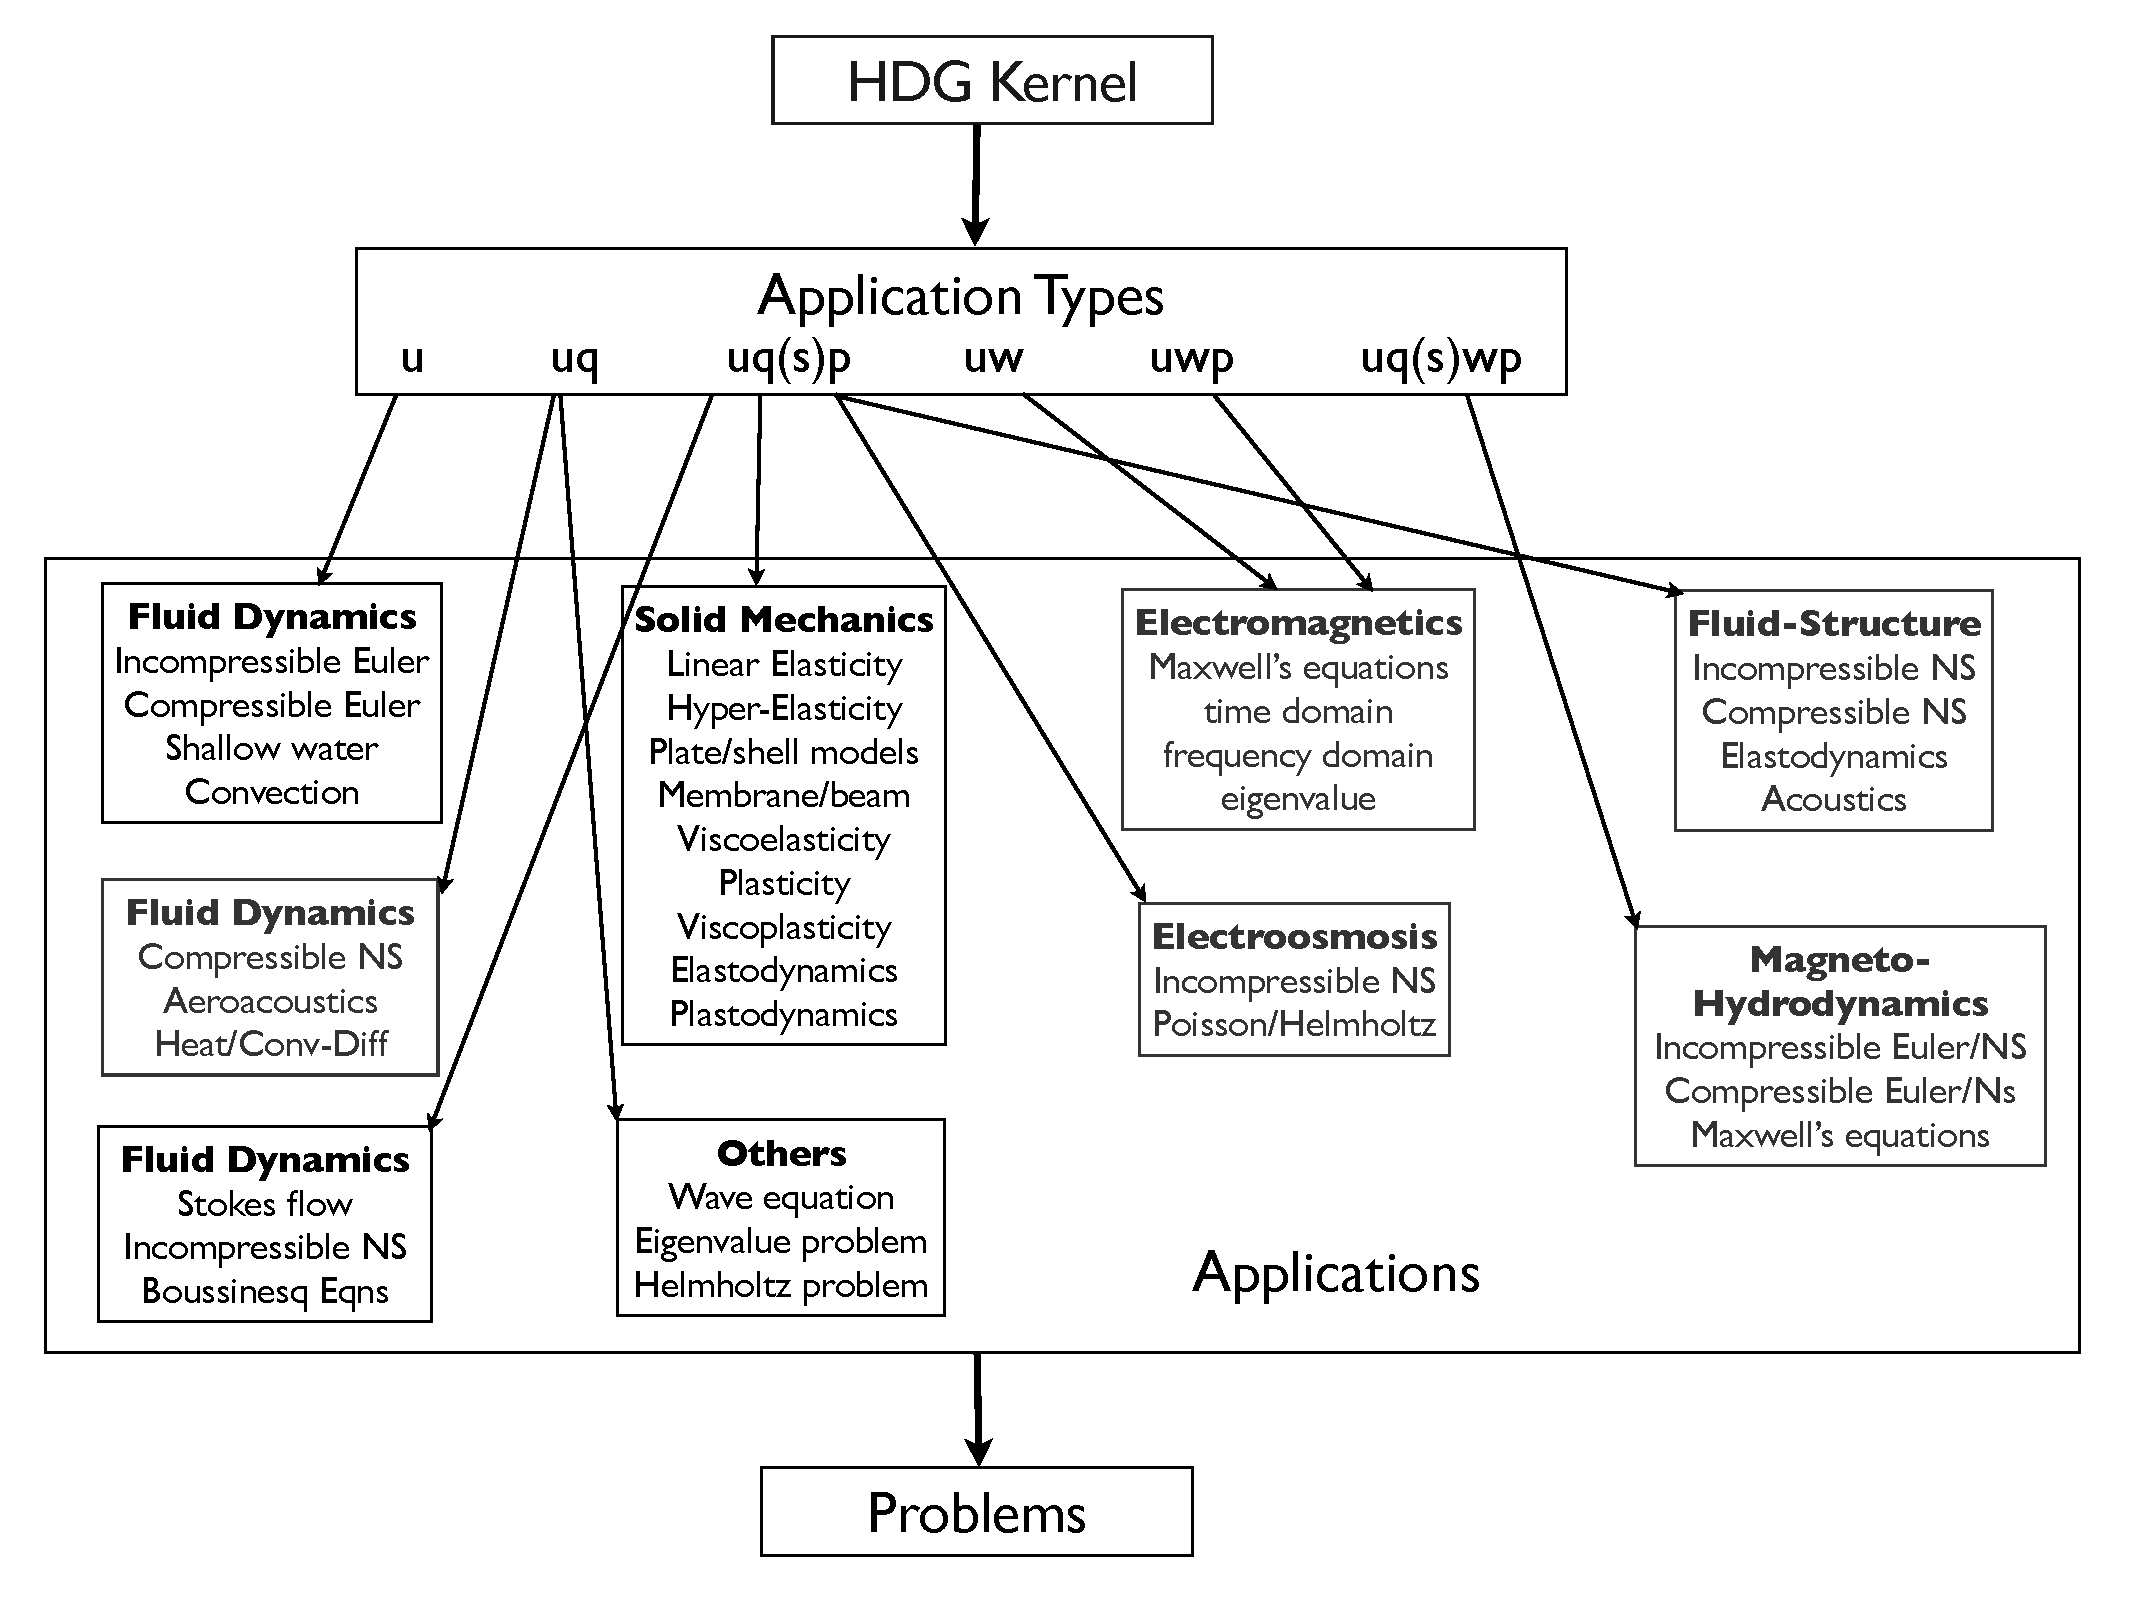
\includegraphics[scale=0.5]{HDGmap.pdf} 
	\end{center}
		\caption{HDG Hierarchy.}
		 \label{HDGmap}
	\end{figure}

\section{HDG Kernel}

HDG Kernel is responsible for forming and solving the linear system for all the Application Types. There are two main functions: 

\begin{itemize}
\item \texttt{hdg\_solve.m} assembles the Jacobian matrix and the Residual vector, and then solves the linear system. \footnote{Need to implement \texttt{globalsolve.m} to solve the linear system.} This function calls \texttt{elemmat.m} and \texttt{localsolve.m} for the assembly of the linear system. The linear system stems from linearization of the nonlinear problem
\begin{equation}
\sum_{K \in \mathcal{T}_h}  \left\langle \bm{\widehat{F}} ({\bm{U}}_h,{\widehat{\bm{u}}}_h) \cdot \bm{n}, \bm{\mu} \right\rangle_{\partial K \backslash \partial \Omega} +  \left\langle \bm{\widehat{F}}^b({\bm{U}}_h,{\widehat{\bm{u}}}_h) \cdot \bm{n} - \bm{g}, \bm{\mu} \right\rangle_{\partial \Omega}  = 0, \quad \forall \bm{\mu} \in \bm{M}_h .
\end{equation}
Here $\bm{\widehat{F}}$ and $\bm{\widehat{F}}^b$ are the interior and boundary fluxes, respectively; and $\bm{g}$ is the boundary data. The definition of the boundary flux  $\bm{\widehat{F}}^b$ depends on the applied boundary conditions and is different on different parts of the boundary $\partial \Omega$.
\item \texttt{elemmat.m} computes the elemental Jacobian matrix and Residual vector by evaluating the following integrals, on the interior faces ${F}$,
\begin{equation}
\begin{array}{rcl}
\mathbb{J}_F & = & \displaystyle \left\langle \Big( \frac{\partial \bm{\widehat{F}}(\overline{\bm{U}}_h,\overline{\widehat{\bm{u}}}_h)}{\partial {\bm{U}}_h} \delta {\bm{U}}^{\delta \bm{\lambda}}_h + \frac{\partial \bm{\widehat{F}}(\overline{\bm{U}}_h,\overline{\widehat{\bm{u}}}_h)}{\partial \widehat{\bm{u}}_h} \delta \widehat{\bm{u}}_h  \Big) \cdot \bm{n}, \bm{\mu} \right\rangle_{F}, \\[3ex]
\mathbb{R}_F & = &  \displaystyle  -\left\langle \bm{\widehat{F}} (\overline{\bm{U}}_h,\overline{\widehat{\bm{u}}}_h) \cdot \bm{n}, \bm{\mu} \right\rangle_{F} - \left\langle \Big( \frac{\partial \bm{\widehat{F}}(\overline{\bm{U}}_h,\overline{\widehat{\bm{u}}}_h)}{\partial {\bm{U}}_h} \delta {\bm{U}}^{\bm{r}}_h  \Big) \cdot \bm{n}, \bm{\mu} \right\rangle_{F};
\end{array}
\end{equation}
on the boundary faces $F \in \partial \Omega$,
\begin{equation}
\begin{array}{rcl}
\mathbb{J}_F & = & \displaystyle \left\langle \Big( \frac{\partial \bm{\widehat{F}}^b(\overline{\bm{U}}_h,\overline{\widehat{\bm{u}}}_h)}{\partial {\bm{U}}_h} \delta {\bm{U}}^{\delta \bm{\lambda}}_h + \frac{\partial \bm{\widehat{F}}^b(\overline{\bm{U}}_h,\overline{\widehat{\bm{u}}}_h)}{\partial \widehat{\bm{u}}_h} \delta \widehat{\bm{u}}_h  \Big) \cdot \bm{n}, \bm{\mu} \right\rangle_{F}, \\[3ex]
\mathbb{R}_F & = &  \displaystyle  -\left\langle \bm{\widehat{F}}^b (\overline{\bm{U}}_h,\overline{\widehat{\bm{u}}}_h) \cdot \bm{n} - \bm{g}, \bm{\mu} \right\rangle_{F} - \left\langle \Big( \frac{\partial \bm{\widehat{F}}^b(\overline{\bm{U}}_h,\overline{\widehat{\bm{u}}}_h)}{\partial {\bm{U}}_h} \delta {\bm{U}}^{\bm{r}}_h  \Big) \cdot \bm{n}, \bm{\mu} \right\rangle_{F} .
\end{array}
\end{equation}
Here $\delta {\bm{U}}^{\delta \bm{\lambda}}_h$ and $\delta {\bm{U}}^{\bm{r}}_h$ are local solutions which are computed in \texttt{localsolve.m}.\footnote{Need to move the call to \texttt{fbou.m} and \texttt{fhat.m} from \texttt{elemmat.m} to \texttt{localsolve.m}}
\item Other functions, \texttt{hdg\_solve\_bdf.m} and \texttt{hdg\_solve\_dirk.m}, call \texttt{hdg\_solve.m} to solve time-dependent problems using BDF and DIRK methods, respectively.
\end{itemize} 

\section{Application Types (PDE Forms)}

Application Types include the local solver to several types of PDEs. The local solver is responsible for computing the local solutions  $\delta {\bm{U}}^{\delta \bm{\lambda}}_h$ and $\delta {\bm{U}}^{\bm{r}}_h$. There are two main functions

\begin{itemize}
\item \texttt{localresid.m} computes the local matrices and vectors on each element.
\item \texttt{localsolve.m} solve the local linear system for $\delta {\bm{U}}^{\delta \bm{\lambda}}_h$ and $\delta {\bm{U}}^{\bm{r}}_h$. 
\end{itemize}

The form of the local linear system depends on the type of PDEs. 

\subsection{$\bm{u}$-Type}

We solve the boundary value problem of the form.
\begin{equation}
\begin{array}{rcll}
- \nabla \cdot \bm{F} (\bm{u}) & = & \bm{f}, & \quad \mbox{in } \Omega, \\
\bm{u} & = & \bm{g}_D, & \quad \mbox{on } \Gamma_D .
\end{array}
\end{equation}
The HDG method seeks $(\bm{u}_h, \widehat{\bm{u}}_h) \in \bm{W}_h \times \bm{M}_h$ such that
\begin{equation}
\begin{array}{rcll}
(\bm{F} (\bm{u}_h), \nabla \bm{w})_{\mathcal{T}_h} - \langle \widehat{\bm{F}} (\bm{u}_h, \widehat{\bm{u}}_h) \cdot \bm{n}, \bm{w} \rangle_{\partial \mathcal{T}_h} & = & (\bm{f}, \bm{w})_{\mathcal{T}_h}, & \quad \forall \bm{w} \in \bm{W}_h, \\[2ex]
\langle \widehat{\bm{F}} (\bm{u}_h, \widehat{\bm{u}}_h) \cdot \bm{n}, \bm{\mu} \rangle_{\partial \mathcal{T}_h \backslash \partial \Omega} + \langle \widehat{\bm{F}}^b(\bm{u}_h, \widehat{\bm{u}}_h) \cdot \bm{n} - \bm{g}, \bm{\mu} \rangle_{\partial \Omega}  & = & 0, & \quad \forall \bm{\mu} \in \bm{M}_h ,
\end{array}
\end{equation}
where
\begin{equation}
\begin{array}{rcll}
\widehat{\bm{F}} (\bm{u}_h, \widehat{\bm{u}}_h) \cdot \bm{n} & = & {\bm{F}} (\widehat{\bm{u}}_h) \cdot \bm{n} - \bm{\mathrm{S}} (\bm{u}_h, \widehat{\bm{u}}_h) (\bm{u}_h - \widehat{\bm{u}}_h), \\[2ex]
\widehat{\bm{F}}^b(\bm{u}_h, \widehat{\bm{u}}_h) \cdot \bm{n} & = & 
\left\{
\begin{array}{ll} 
\widehat{\bm{u}}_h, & \quad  \mbox{on } \Gamma_D, \\
-\bm{\mathrm{S}} (\bm{u}_h, \widehat{\bm{u}}_h) (\bm{u}_h - \widehat{\bm{u}}_h), & \quad \mbox{on }  \partial \Omega \backslash \Gamma_D,  
\end{array}
\right. \\[3ex]
\bm{g} & = & 
\left\{
\begin{array}{ll} 
\bm{g}_D, & \quad  \mbox{on } \Gamma_D, \\
\bm{0}, & \quad \mbox{on }  \partial \Omega \backslash \Gamma_D .  
\end{array}
\right.
\end{array}
\end{equation}
Linearization of the first equation of (5) gives
\begin{equation}
(\partial_{\bm{u}} \bm{F} (\overline{\bm{u}}_h) \delta \bm{u}_h, \nabla \bm{w})_{\mathcal{T}_h} - \langle (\partial_{\bm{u}} \widehat{\bm{F}} (\overline{\bm{u}}_h, \overline{\widehat{\bm{u}}}_h) \delta \bm{u}_h + \partial_{\widehat{\bm{u}}} \widehat{\bm{F}} (\overline{\bm{u}}_h, \overline{\widehat{\bm{u}}}_h) \delta \widehat{\bm{u}}_h) \cdot \bm{n}, \bm{w} \rangle_{\partial \mathcal{T}_h}  =  \bm{r}(\bm{w})_{\mathcal{T}_h},  \quad \forall \bm{w} \in \bm{W}_h,
\end{equation}
where
\begin{equation}
\bm{r}(\bm{w})_{\mathcal{T}_h} = (\bm{f}, \bm{w})_{\mathcal{T}_h} - (\bm{F} (\overline{\bm{u}}_h), \nabla \bm{w})_{\mathcal{T}_h} + \langle \widehat{\bm{F}} (\overline{\bm{u}}_h, \overline{\widehat{\bm{u}}}_h) \cdot \bm{n}, \bm{w} \rangle_{\partial \mathcal{T}_h} .
\end{equation}
As a result, $\delta \bm{u}_h^{\bm{r}}$ is the solution of
\begin{equation}
(\partial_{\bm{u}} \bm{F} (\overline{\bm{u}}_h) \delta \bm{u}_h, \nabla \bm{w})_{\mathcal{T}_h} - \langle (\partial_{\bm{u}} \widehat{\bm{F}} (\overline{\bm{u}}_h, \overline{\widehat{\bm{u}}}_h) \delta \bm{u}_h, \bm{w} \rangle_{\partial \mathcal{T}_h}  =  \bm{r}(\bm{w})_{\mathcal{T}_h},  \quad \forall \bm{w} \in \bm{W}_h.
\end{equation}
And $\delta \bm{u}_h^{\delta \bm{\lambda}}$ is the solution of
\begin{equation}
(\partial_{\bm{u}} \bm{F} (\overline{\bm{u}}_h) \delta \bm{u}_h, \nabla \bm{w})_{\mathcal{T}_h} - \langle (\partial_{\bm{u}} \widehat{\bm{F}} (\overline{\bm{u}}_h, \overline{\widehat{\bm{u}}}_h) \delta \bm{u}_h, \bm{w} \rangle_{\partial \mathcal{T}_h}  = \langle (\partial_{\widehat{\bm{u}}} \widehat{\bm{F}} (\overline{\bm{u}}_h, \overline{\widehat{\bm{u}}}_h) \delta \bm{\lambda}, \bm{w} \rangle_{\partial \mathcal{T}_h}, \quad \forall \bm{w} \in \bm{W}_h.
\end{equation}
The Eqns (9) and (10) define the local solver.

%\begin{equation}
%\begin{array}{rcll}
%(\bm{q}_h, \bm{v}) - (\bm{F}(\bm{u}_h), \bm{v}) & = & 0 , & \\
%(\bm{q}_h, \nabla \bm{w})_{\mathcal{T}_h} - \langle \widehat{\bm{F}} (\bm{u}_h, \widehat{\bm{u}}_h) \cdot \bm{n}, \bm{w} \rangle_{\partial \mathcal{T}_h} & = & (\bm{f}, \bm{w})_{\mathcal{T}_h}, & \quad \forall \bm{w} \in \bm{W}_h, \\[2ex]
%\langle \widehat{\bm{F}} (\bm{u}_h, \widehat{\bm{u}}_h) \cdot \bm{n}, \bm{\mu} \rangle_{\partial \mathcal{T}_h \backslash \partial \Omega} + \langle \widehat{\bm{F}}^b(\bm{u}_h, \widehat{\bm{u}}_h) \cdot \bm{n} - \bm{g}, \bm{\mu} \rangle_{\partial \Omega}  & = & 0, & \quad \forall \bm{\mu} \in \bm{M}_h ,
%\end{array}
%\end{equation}

Next, we consider the time-dependent problem
\begin{equation}
\begin{array}{rcll}
\displaystyle \frac{\partial \bm{u}}{\partial t} - \nabla \cdot \bm{F} (\bm{u}) & = & \bm{f}, & \quad \mbox{in } \Omega, \\
\bm{u} & = & \bm{g}_D, & \quad \mbox{on } \Gamma_D .
\end{array}
\end{equation}
The HDG method seeks $(\bm{u}_h, \widehat{\bm{u}}_h) \in \bm{W}_h \times \bm{M}_h$ such that
\begin{equation}
\begin{array}{rcll}
\displaystyle \Big(\frac{\bm{u}_h}{\Delta t}, \bm{w} \Big)_{\mathcal{T}_h} + (\bm{F} (\bm{u}_h), \nabla \bm{w})_{\mathcal{T}_h} - \langle \widehat{\bm{F}} (\bm{u}_h, \widehat{\bm{u}}_h) \cdot \bm{n}, \bm{w} \rangle_{\partial \mathcal{T}_h} & = & (\bm{f}, \bm{w})_{\mathcal{T}_h} + \displaystyle \Big(\frac{\bm{u}_h^{k-1}}{\Delta t}, \bm{w} \Big)_{\mathcal{T}_h}, & \quad \forall \bm{w} \in \bm{W}_h, \\[2ex]
\langle \widehat{\bm{F}} (\bm{u}_h, \widehat{\bm{u}}_h) \cdot \bm{n}, \bm{\mu} \rangle_{\partial \mathcal{T}_h \backslash \partial \Omega} + \langle \widehat{\bm{F}}^b(\bm{u}_h, \widehat{\bm{u}}_h) \cdot \bm{n} - \bm{g}, \bm{\mu} \rangle_{\partial \Omega}  & = & 0, & \quad \forall \bm{\mu} \in \bm{M}_h .
\end{array}
\end{equation}
Linearization of the first equation of (12) gives
\begin{multline}
\displaystyle \Big( \frac{\delta \bm{u}_h}{\Delta t}, \bm{w} \Big)_{\mathcal{T}_h}  + (\partial_{\bm{u}} \bm{F} (\overline{\bm{u}}_h) \delta \bm{u}_h, \nabla \bm{w})_{\mathcal{T}_h} - \langle (\partial_{\bm{u}} \widehat{\bm{F}} (\overline{\bm{u}}_h, \overline{\widehat{\bm{u}}}_h) \delta \bm{u}_h + \partial_{\widehat{\bm{u}}} \widehat{\bm{F}} (\overline{\bm{u}}_h, \overline{\widehat{\bm{u}}}_h) \delta \widehat{\bm{u}}_h) \cdot \bm{n}, \bm{w} \rangle_{\partial \mathcal{T}_h}\\  =  \bm{r}(\bm{w})_{\mathcal{T}_h},  \quad \forall \bm{w} \in \bm{W}_h,
\end{multline}
where
\begin{equation}
\bm{r}(\bm{w})_{\mathcal{T}_h} = (\bm{f}, \bm{w})_{\mathcal{T}_h} + \displaystyle \Big(\frac{\bm{u}_h^{k-1}}{\Delta t}, \bm{w} \Big)_{\mathcal{T}_h} - \Big(\frac{\overline{\bm{u}}_h}{\Delta t}, \bm{w} \Big)_{\mathcal{T}_h} - (\bm{F} (\overline{\bm{u}}_h), \nabla \bm{w})_{\mathcal{T}_h} + \langle \widehat{\bm{F}} (\overline{\bm{u}}_h, \overline{\widehat{\bm{u}}}_h) \cdot \bm{n}, \bm{w} \rangle_{\partial \mathcal{T}_h} .
\end{equation}
As a result, $\delta \bm{u}_h^{\bm{r}}$ is the solution of
\begin{equation}
\displaystyle \Big( \frac{\delta \bm{u}_h}{\Delta t}, \bm{w} \Big)_{\mathcal{T}_h} + (\partial_{\bm{u}} \bm{F} (\overline{\bm{u}}_h) \delta \bm{u}_h, \nabla \bm{w})_{\mathcal{T}_h} - \langle (\partial_{\bm{u}} \widehat{\bm{F}} (\overline{\bm{u}}_h, \overline{\widehat{\bm{u}}}_h) \delta \bm{u}_h, \bm{w} \rangle_{\partial \mathcal{T}_h}  =  \bm{r}(\bm{w})_{\mathcal{T}_h},  \quad \forall \bm{w} \in \bm{W}_h.
\end{equation}
And $\delta \bm{u}_h^{\delta \bm{\lambda}}$ is the solution of
\begin{equation}
\displaystyle \Big( \frac{\delta \bm{u}_h}{\Delta t}, \bm{w} \Big)_{\mathcal{T}_h} + (\partial_{\bm{u}} \bm{F} (\overline{\bm{u}}_h) \delta \bm{u}_h, \nabla \bm{w})_{\mathcal{T}_h} - \langle (\partial_{\bm{u}} \widehat{\bm{F}} (\overline{\bm{u}}_h, \overline{\widehat{\bm{u}}}_h) \delta \bm{u}_h, \bm{w} \rangle_{\partial \mathcal{T}_h}  = \langle (\partial_{\widehat{\bm{u}}} \widehat{\bm{F}} (\overline{\bm{u}}_h, \overline{\widehat{\bm{u}}}_h) \delta \bm{\lambda}, \bm{w} \rangle_{\partial \mathcal{T}_h}, \quad \forall \bm{w} \in \bm{W}_h.
\end{equation}
The Eqns (15) and (16) define the local solver.

\subsection{$\bm{uq}$-Type}

We solve the boundary value problem of the form.
\begin{equation}
\begin{array}{rcll}
\bm{q} - \nabla \bm{u}  & = & \bm{0} , & \quad \mbox{in } \Omega, \\
- \nabla \cdot \bm{F} (\bm{u},\bm{q}) & = & \bm{f}, & \quad \mbox{in } \Omega, \\
\bm{u} & = & \bm{g}_D, & \quad \mbox{on } \Gamma_D , \\
\bm{B}^n(\bm{u},\bm{q}) \cdot \bm{n} & = & \bm{g}_N, & \quad \mbox{on } \Gamma_N .
\end{array}
\end{equation}
The HDG method seeks $(\bm{u}_h,\bm{q}_h,\widehat{\bm{u}}_h) \in \bm{W}_h \times \bm{V}_h \times \bm{M}_h$ such that
\begin{equation}
\begin{array}{rcll}
(\bm{q}_h, \bm{v})_{\mathcal{T}_h} + (\bm{u}_h, \nabla \cdot \bm{v})_{\mathcal{T}_h} - \langle \widehat{\bm{u}}_h, \bm{v} \cdot \bm{n} \rangle_{\partial \mathcal{T}_h}  & = & \bm{0}, & \quad \forall \bm{v} \in \bm{V}_h, \\[2ex] 
(\bm{F} (\bm{u}_h,\bm{q}_h), \nabla \bm{w})_{\mathcal{T}_h} - \langle \widehat{\bm{F}} (\bm{u}_h, \bm{q}_h,\widehat{\bm{u}}_h) \cdot \bm{n}, \bm{w} \rangle_{\partial \mathcal{T}_h} & = & (\bm{f}, \bm{w})_{\mathcal{T}_h}, & \quad \forall \bm{w} \in \bm{W}_h, \\[2ex]
\langle \widehat{\bm{F}} (\bm{u}_h,\bm{q}_h, \widehat{\bm{u}}_h) \cdot \bm{n}, \bm{\mu} \rangle_{\partial \mathcal{T}_h \backslash \partial \Omega} + \langle \widehat{\bm{F}}^b(\bm{u}_h, \bm{q}_h, \widehat{\bm{u}}_h) \cdot \bm{n} - \bm{g}, \bm{\mu} \rangle_{\partial \Omega}  & = & 0, & \quad \forall \bm{\mu} \in \bm{M}_h ,
\end{array}
\end{equation}
where
\begin{equation}
\begin{array}{rcll}
\widehat{\bm{F}} (\bm{u}_h, \bm{q}_h, \widehat{\bm{u}}_h) \cdot \bm{n} & = & {\bm{F}} (\widehat{\bm{u}}_h,\bm{q}_h) \cdot \bm{n} - \bm{\mathrm{S}} (\bm{u}_h, \bm{q}_h, \widehat{\bm{u}}_h) (\bm{u}_h - \widehat{\bm{u}}_h), \\[2ex]
\widehat{\bm{F}}^b(\bm{u}_h, \bm{q}_h, \widehat{\bm{u}}_h) \cdot \bm{n} & = & 
\left\{
\begin{array}{ll} 
\widehat{\bm{u}}_h, & \quad  \mbox{on } \Gamma_D, \\
\bm{B}^n(\widehat{\bm{u}}_h,\bm{q}_h) \cdot \bm{n} -\bm{\mathrm{S}} (\bm{u}_h, \bm{q}_h,\widehat{\bm{u}}_h) (\bm{u}_h - \widehat{\bm{u}}_h), & \quad \mbox{on }   \Gamma_N,  
\end{array}
\right. \\[3ex]
\bm{g} & = & 
\left\{
\begin{array}{ll} 
\bm{g}_D, & \quad  \mbox{on } \Gamma_D, \\
\bm{g}_N, & \quad \mbox{on }   \Gamma_N .  
\end{array}
\right.
\end{array}
\end{equation}
Linearization of the first two equations of (18) gives
\begin{equation}
\begin{array}{rcll}
(\delta \bm{q}_h, \bm{v})_{\mathcal{T}_h} + (\delta \bm{u}_h, \nabla \cdot \bm{v})_{\mathcal{T}_h} - \langle \delta \widehat{\bm{u}}_h, \bm{v} \cdot \bm{n} \rangle_{\partial \mathcal{T}_h}  & = & \bm{r}(\bm{v}), & \quad \forall \bm{v} \in \bm{V}_h, \\[2ex] 
(\partial_{\bm{u}} \bm{F} (\overline{\bm{U}}_h) \delta \bm{u}_h + \partial_{\bm{q}} \bm{F} (\overline{\bm{U}}_h) \delta \bm{q}_h, \nabla \bm{w})_{\mathcal{T}_h} & & \\[2ex]
- \langle (\partial_{\bm{u}} \widehat{\bm{F}} (\overline{\bm{U}}_h,\overline{\widehat{\bm{u}}}_h) \delta \bm{u}_h + \partial_{{\bm{q}}} \widehat{\bm{F}} (\overline{\bm{U}}_h,\overline{\widehat{\bm{u}}}_h) \delta {\bm{q}}_h) \cdot \bm{n}, \bm{w} \rangle_{\partial \mathcal{T}_h} & & \\[2ex]
 - \langle (\partial_{\widehat{\bm{u}}} \widehat{\bm{F}} (\overline{\bm{U}}_h, \overline{\widehat{\bm{u}}}_h) \delta \widehat{\bm{u}}_h) \cdot \bm{n}, \bm{w} \rangle_{\partial \mathcal{T}_h}   & = &  \bm{r}(\bm{w})_{\mathcal{T}_h},  & \quad \forall \bm{w} \in \bm{W}_h,
\end{array}
\end{equation}
where
\begin{equation}
\begin{array}{rcl}
 \bm{r}(\bm{v}) & = & -(\overline{\bm{q}}_h, \bm{v})_{\mathcal{T}_h} - (\overline{\bm{u}}_h, \nabla \cdot \bm{v})_{\mathcal{T}_h} + \langle \overline{\widehat{\bm{u}}}_h, \bm{v} \cdot \bm{n} \rangle_{\partial \mathcal{T}_h},  \\[2ex]
\bm{r}(\bm{w})_{\mathcal{T}_h} & = & (\bm{f}, \bm{w})_{\mathcal{T}_h} - (\bm{F} (\overline{\bm{U}}_h), \nabla \bm{w})_{\mathcal{T}_h} + \langle \widehat{\bm{F}} (\overline{\bm{U}}_h, \overline{\widehat{\bm{u}}}_h) \cdot \bm{n}, \bm{w} \rangle_{\partial \mathcal{T}_h} .
\end{array}
\end{equation}
As a result, $(\delta \bm{u}_h^{\bm{r}},\delta \bm{q}_h^{\bm{r}})$ is the solution of
\begin{equation}
\begin{array}{rcll}
(\delta \bm{q}_h, \bm{v})_{\mathcal{T}_h} + (\delta \bm{u}_h, \nabla \cdot \bm{v})_{\mathcal{T}_h}  & = & \bm{r}(\bm{v}), & \quad \forall \bm{v} \in \bm{V}_h, \\[2ex] 
(\partial_{\bm{u}} \bm{F} (\overline{\bm{U}}_h) \delta \bm{u}_h + \partial_{\bm{q}} \bm{F} (\overline{\bm{U}}_h) \delta \bm{q}_h, \nabla \bm{w})_{\mathcal{T}_h} & & \\[2ex]
- \langle (\partial_{\bm{u}} \widehat{\bm{F}} (\overline{\bm{U}}_h, \overline{\widehat{\bm{u}}}_h) \delta \bm{u}_h + \partial_{{\bm{q}}} \widehat{\bm{F}} (\overline{\bm{U}}_h, \overline{\widehat{\bm{u}}}_h) \delta {\bm{q}}_h) \cdot \bm{n}, \bm{w} \rangle_{\partial \mathcal{T}_h}  & = &  \bm{r}(\bm{w})_{\mathcal{T}_h},  & \quad \forall \bm{w} \in \bm{W}_h,
\end{array}
\end{equation}
And $(\delta \bm{u}_h^{\delta \bm{\lambda}},\delta \bm{q}_h^{\delta \bm{\lambda}})$ is the solution of
\begin{equation}
\begin{array}{rcll}
(\delta \bm{q}_h, \bm{v})_{\mathcal{T}_h} + (\delta \bm{u}_h, \nabla \cdot \bm{v})_{\mathcal{T}_h}  & = & \langle \delta {\bm{\lambda}}, \bm{v} \cdot \bm{n} \rangle_{\partial \mathcal{T}_h} , & \quad \forall \bm{v} \in \bm{V}_h, \\[2ex] 
(\partial_{\bm{u}} \bm{F} (\overline{\bm{U}}_h) \delta \bm{u}_h + \partial_{\bm{q}} \bm{F} (\overline{\bm{U}}_h) \delta \bm{q}_h, \nabla \bm{w})_{\mathcal{T}_h} & & \\[2ex]
- \langle (\partial_{\bm{u}} \widehat{\bm{F}} (\overline{\bm{U}}_h, \overline{\widehat{\bm{u}}}_h) \delta \bm{u}_h + \partial_{{\bm{q}}} \widehat{\bm{F}} (\overline{\bm{U}}_h, \overline{\widehat{\bm{u}}}_h) \delta {\bm{q}}_h) \cdot \bm{n}, \bm{w} \rangle_{\partial \mathcal{T}_h}  & = &  \langle (\partial_{\widehat{\bm{u}}} \widehat{\bm{F}} (\overline{\bm{U}}_h, \overline{\widehat{\bm{u}}}_h) \delta {\bm{\lambda}}) \cdot \bm{n}, \bm{w} \rangle_{\partial \mathcal{T}_h},  & \quad \forall \bm{w} \in \bm{W}_h,
\end{array}
\end{equation}
The Eqns (22) and (23) define the local solver.

We consider the time-dependent problem
\begin{equation}
\begin{array}{rcll}
\bm{q} - \nabla \bm{u}  & = & \bm{0} , & \quad \mbox{in } \Omega, \\
\displaystyle \frac{\partial \bm{u}}{\partial t}  - \nabla \cdot \bm{F} (\bm{u},\bm{q}) & = & \bm{f}, & \quad \mbox{in } \Omega, \\
\bm{u} & = & \bm{g}_D, & \quad \mbox{on } \Gamma_D , \\
\bm{B}^n(\bm{u},\bm{q}) \cdot \bm{n} & = & \bm{g}_N, & \quad \mbox{on } \Gamma_N .
\end{array}
\end{equation}
The HDG method seeks $(\bm{u}_h,\bm{q}_h,\widehat{\bm{u}}_h) \in \bm{W}_h \times \bm{V}_h \times \bm{M}_h$ such that
\begin{equation}
\begin{array}{rcll}
(\bm{q}_h, \bm{v})_{\mathcal{T}_h} + (\bm{u}_h, \nabla \cdot \bm{v})_{\mathcal{T}_h} - \langle \widehat{\bm{u}}_h, \bm{v} \cdot \bm{n} \rangle_{\partial \mathcal{T}_h}  & = & \bm{0}, & \quad \forall \bm{v} \in \bm{V}_h, \\[2ex] 
\displaystyle \Big(\frac{\bm{u}_h}{\Delta t}, \bm{w} \Big)_{\mathcal{T}_h} + (\bm{F} (\bm{u}_h,\bm{q}_h), \nabla \bm{w})_{\mathcal{T}_h} - \langle \widehat{\bm{F}} (\bm{u}_h, \bm{q}_h,\widehat{\bm{u}}_h) \cdot \bm{n}, \bm{w} \rangle_{\partial \mathcal{T}_h} & = & (\bm{f}, \bm{w})_{\mathcal{T}_h} + \displaystyle \Big(\frac{\bm{u}_h^{k-1}}{\Delta t}, \bm{w} \Big)_{\mathcal{T}_h}, & \quad \forall \bm{w} \in \bm{W}_h, \\[2ex]
\langle \widehat{\bm{F}} (\bm{u}_h,\bm{q}_h, \widehat{\bm{u}}_h) \cdot \bm{n}, \bm{\mu} \rangle_{\partial \mathcal{T}_h \backslash \partial \Omega} + \langle \widehat{\bm{F}}^b(\bm{u}_h, \bm{q}_h, \widehat{\bm{u}}_h) \cdot \bm{n} - \bm{g}, \bm{\mu} \rangle_{\partial \Omega}  & = & 0, & \quad \forall \bm{\mu} \in \bm{M}_h ,
\end{array}
\end{equation}
Linearization of the first two equations of (25) gives
\begin{equation}
\begin{array}{rcll}
(\delta \bm{q}_h, \bm{v})_{\mathcal{T}_h} + (\delta \bm{u}_h, \nabla \cdot \bm{v})_{\mathcal{T}_h} - \langle \delta \widehat{\bm{u}}_h, \bm{v} \cdot \bm{n} \rangle_{\partial \mathcal{T}_h}  & = & \bm{r}(\bm{v}), & \quad \forall \bm{v} \in \bm{V}_h, \\[2ex] 
\displaystyle \Big(\frac{\delta \bm{u}_h}{\Delta t}, \bm{w} \Big)_{\mathcal{T}_h} + (\partial_{\bm{u}} \bm{F} (\overline{\bm{U}}_h) \delta \bm{u}_h + \partial_{\bm{q}} \bm{F} (\overline{\bm{U}}_h) \delta \bm{q}_h, \nabla \bm{w})_{\mathcal{T}_h} & & \\[2ex]
 - \langle (\partial_{\bm{u}} \widehat{\bm{F}} (\overline{\bm{U}}_h, \overline{\widehat{\bm{u}}}_h) \delta \bm{u}_h + \partial_{{\bm{q}}} \widehat{\bm{F}} (\overline{\bm{U}}_h, \overline{\widehat{\bm{u}}}_h) \delta {\bm{q}}_h) \cdot \bm{n}, \bm{w} \rangle_{\partial \mathcal{T}_h} & & \\[2ex]
 - \langle (\partial_{\widehat{\bm{u}}} \widehat{\bm{F}} (\overline{\bm{U}}_h, \overline{\widehat{\bm{u}}}_h) \delta \widehat{\bm{u}}_h) \cdot \bm{n}, \bm{w} \rangle_{\partial \mathcal{T}_h}   & = &  \bm{r}(\bm{w})_{\mathcal{T}_h},  & \quad \forall \bm{w} \in \bm{W}_h,
\end{array}
\end{equation}
where
\begin{equation}
\begin{array}{rcl}
 \bm{r}(\bm{v}) & = & -(\overline{\bm{q}}_h, \bm{v})_{\mathcal{T}_h} - (\overline{\bm{u}}_h, \nabla \cdot \bm{v})_{\mathcal{T}_h} + \langle \overline{\widehat{\bm{u}}}_h, \bm{v} \cdot \bm{n} \rangle_{\partial \mathcal{T}_h},  \\[2ex]
\bm{r}(\bm{w})_{\mathcal{T}_h} & = & (\bm{f}, \bm{w})_{\mathcal{T}_h} + \displaystyle \Big(\frac{\bm{u}_h^{k-1}}{\Delta t}, \bm{w} \Big)_{\mathcal{T}_h} - \Big(\frac{ \overline{\bm{u}}_h}{\Delta t}, \bm{w} \Big)_{\mathcal{T}_h}- (\bm{F} (\overline{\bm{U}}_h), \nabla \bm{w})_{\mathcal{T}_h} + \langle \widehat{\bm{F}} (\overline{\bm{U}}_h, \overline{\widehat{\bm{u}}}_h) \cdot \bm{n}, \bm{w} \rangle_{\partial \mathcal{T}_h} .
\end{array}
\end{equation}
As a result, $(\delta \bm{u}_h^{\bm{r}},\delta \bm{q}_h^{\bm{r}})$ is the solution of
\begin{equation}
\begin{array}{rcll}
(\delta \bm{q}_h, \bm{v})_{\mathcal{T}_h} + (\delta \bm{u}_h, \nabla \cdot \bm{v})_{\mathcal{T}_h}  & = & \bm{r}(\bm{v}), & \quad \forall \bm{v} \in \bm{V}_h, \\[2ex] 
\displaystyle \Big(\frac{\delta \bm{u}_h}{\Delta t}, \bm{w} \Big)_{\mathcal{T}_h} + (\partial_{\bm{u}} \bm{F} (\overline{\bm{U}}_h) \delta \bm{u}_h + \partial_{\bm{q}} \bm{F} (\overline{\bm{U}}_h) \delta \bm{q}_h, \nabla \bm{w})_{\mathcal{T}_h} & & \\[2ex]
- \langle (\partial_{\bm{u}} \widehat{\bm{F}} (\overline{\bm{U}}_h, \overline{\widehat{\bm{u}}}_h) \delta \bm{u}_h + \partial_{{\bm{q}}} \widehat{\bm{F}} (\overline{\bm{U}}_h, \overline{\widehat{\bm{u}}}_h) \delta {\bm{q}}_h) \cdot \bm{n}, \bm{w} \rangle_{\partial \mathcal{T}_h}  & = &  \bm{r}(\bm{w})_{\mathcal{T}_h},  & \quad \forall \bm{w} \in \bm{W}_h,
\end{array}
\end{equation}
And $(\delta \bm{u}_h^{\delta \bm{\lambda}},\delta \bm{q}_h^{\delta \bm{\lambda}})$ is the solution of
\begin{equation}
\begin{array}{rcll}
(\delta \bm{q}_h, \bm{v})_{\mathcal{T}_h} + (\delta \bm{u}_h, \nabla \cdot \bm{v})_{\mathcal{T}_h}  & = & \langle \delta {\bm{\lambda}}, \bm{v} \cdot \bm{n} \rangle_{\partial \mathcal{T}_h} , & \quad \forall \bm{v} \in \bm{V}_h, \\[2ex] 
\displaystyle \Big(\frac{\delta \bm{u}_h}{\Delta t}, \bm{w} \Big)_{\mathcal{T}_h} + (\partial_{\bm{u}} \bm{F} (\overline{\bm{U}}_h) \delta \bm{u}_h + \partial_{\bm{q}} \bm{F} (\overline{\bm{U}}_h) \delta \bm{q}_h, \nabla \bm{w})_{\mathcal{T}_h} & & \\[2ex]
- \langle (\partial_{\bm{u}} \widehat{\bm{F}} (\overline{\bm{U}}_h, \overline{\widehat{\bm{u}}}_h) \delta \bm{u}_h + \partial_{{\bm{q}}} \widehat{\bm{F}} (\overline{\bm{U}}_h, \overline{\widehat{\bm{u}}}_h) \delta {\bm{q}}_h) \cdot \bm{n}, \bm{w} \rangle_{\partial \mathcal{T}_h}  & = &  \langle (\partial_{\widehat{\bm{u}}} \widehat{\bm{F}} (\overline{\bm{U}}_h, \overline{\widehat{\bm{u}}}_h) \delta {\bm{\lambda}}) \cdot \bm{n}, \bm{w} \rangle_{\partial \mathcal{T}_h},  & \quad \forall \bm{w} \in \bm{W}_h,
\end{array}
\end{equation}
The Eqns (28) and (29) define the local solver.


We consider the wave propagation problem
\begin{equation}
\begin{array}{rcll}
\displaystyle \frac{\partial \bm{q}}{\partial t} - \nabla \bm{u}  & = & \bm{0} , & \quad \mbox{in } \Omega, \\
\displaystyle \frac{\partial \bm{u}}{\partial t}  - \nabla \cdot \bm{F} (\bm{u},\bm{q}) & = & \bm{f}, & \quad \mbox{in } \Omega, \\
\bm{u} & = & \bm{g}_D, & \quad \mbox{on } \Gamma_D , \\
\bm{B}^n(\bm{u},\bm{q}) \cdot \bm{n} & = & \bm{g}_N, & \quad \mbox{on } \Gamma_N .
\end{array}
\end{equation}
The HDG method seeks $(\bm{u}_h,\bm{q}_h,\widehat{\bm{u}}_h) \in \bm{W}_h \times \bm{V}_h \times \bm{M}_h$ such that
\begin{equation}
\begin{array}{rcll}
\displaystyle \Big(\frac{\bm{q}_h}{\Delta t}, \bm{v} \Big)_{\mathcal{T}_h} + (\bm{u}_h, \nabla \cdot \bm{v})_{\mathcal{T}_h} - \langle \widehat{\bm{u}}_h, \bm{v} \cdot \bm{n} \rangle_{\partial \mathcal{T}_h}  & = & \displaystyle \Big(\frac{\bm{q}_h^{k-1}}{\Delta t}, \bm{v} \Big)_{\mathcal{T}_h}, & \quad \forall \bm{v} \in \bm{V}_h, \\[2ex] 
\displaystyle \Big(\frac{\bm{u}_h}{\Delta t}, \bm{w} \Big)_{\mathcal{T}_h} + (\bm{F} (\bm{u}_h,\bm{q}_h), \nabla \bm{w})_{\mathcal{T}_h} - \langle \widehat{\bm{F}} (\bm{u}_h, \bm{q}_h,\widehat{\bm{u}}_h) \cdot \bm{n}, \bm{w} \rangle_{\partial \mathcal{T}_h} & = & (\bm{f}, \bm{w})_{\mathcal{T}_h} + \displaystyle \Big(\frac{\bm{u}_h^{k-1}}{\Delta t}, \bm{w} \Big)_{\mathcal{T}_h}, & \quad \forall \bm{w} \in \bm{W}_h, \\[2ex]
\langle \widehat{\bm{F}} (\bm{u}_h,\bm{q}_h, \widehat{\bm{u}}_h) \cdot \bm{n}, \bm{\mu} \rangle_{\partial \mathcal{T}_h \backslash \partial \Omega} + \langle \widehat{\bm{F}}^b(\bm{u}_h, \bm{q}_h, \widehat{\bm{u}}_h) \cdot \bm{n} - \bm{g}, \bm{\mu} \rangle_{\partial \Omega}  & = & 0, & \quad \forall \bm{\mu} \in \bm{M}_h ,
\end{array}
\end{equation}
Linearization of the first two equations of (31) gives
\begin{equation}
\begin{array}{rcll}
\displaystyle \Big(\frac{\delta \bm{q}_h}{\Delta t}, \bm{v} \Big)_{\mathcal{T}_h} + (\delta \bm{u}_h, \nabla \cdot \bm{v})_{\mathcal{T}_h} - \langle \delta \widehat{\bm{u}}_h, \bm{v} \cdot \bm{n} \rangle_{\partial \mathcal{T}_h}  & = & \bm{r}(\bm{v}), & \quad \forall \bm{v} \in \bm{V}_h, \\[2ex] 
\displaystyle \Big(\frac{\delta \bm{u}_h}{\Delta t}, \bm{w} \Big)_{\mathcal{T}_h} + (\partial_{\bm{u}} \bm{F} (\overline{\bm{U}}_h) \delta \bm{u}_h + \partial_{\bm{q}} \bm{F} (\overline{\bm{U}}_h) \delta \bm{q}_h, \nabla \bm{w})_{\mathcal{T}_h} & & \\[2ex]
 - \langle (\partial_{\bm{u}} \widehat{\bm{F}} (\overline{\bm{U}}_h, \overline{\widehat{\bm{u}}}_h) \delta \bm{u}_h + \partial_{{\bm{q}}} \widehat{\bm{F}} (\overline{\bm{U}}_h, \overline{\widehat{\bm{u}}}_h) \delta {\bm{q}}_h) \cdot \bm{n}, \bm{w} \rangle_{\partial \mathcal{T}_h} & & \\[2ex]
 - \langle (\partial_{\widehat{\bm{u}}} \widehat{\bm{F}} (\overline{\bm{U}}_h, \overline{\widehat{\bm{u}}}_h) \delta \widehat{\bm{u}}_h) \cdot \bm{n}, \bm{w} \rangle_{\partial \mathcal{T}_h}   & = &  \bm{r}(\bm{w})_{\mathcal{T}_h},  & \quad \forall \bm{w} \in \bm{W}_h,
\end{array}
\end{equation}
where
\begin{equation}
\begin{array}{rcl}
 \bm{r}(\bm{v}) & = & \displaystyle \Big(\frac{\bm{q}_h^{k-1}}{\Delta t}, \bm{v} \Big)_{\mathcal{T}_h} - \Big(\frac{\overline{\bm{q}}_h}{\Delta t}, \bm{v}\Big)_{\mathcal{T}_h} - (\overline{\bm{u}}_h, \nabla \cdot \bm{v})_{\mathcal{T}_h} + \langle \overline{\widehat{\bm{u}}}_h, \bm{v} \cdot \bm{n} \rangle_{\partial \mathcal{T}_h},  \\[2ex]
\bm{r}(\bm{w})_{\mathcal{T}_h} & = & (\bm{f}, \bm{w})_{\mathcal{T}_h} + \displaystyle \Big(\frac{\bm{u}_h^{k-1}}{\Delta t}, \bm{w} \Big)_{\mathcal{T}_h} - \Big(\frac{ \overline{\bm{u}}_h}{\Delta t}, \bm{w} \Big)_{\mathcal{T}_h}- (\bm{F} (\overline{\bm{U}}_h), \nabla \bm{w})_{\mathcal{T}_h} + \langle \widehat{\bm{F}} (\overline{\bm{U}}_h, \overline{\widehat{\bm{u}}}_h) \cdot \bm{n}, \bm{w} \rangle_{\partial \mathcal{T}_h} .
\end{array}
\end{equation}
As a result, $(\delta \bm{u}_h^{\bm{r}},\delta \bm{q}_h^{\bm{r}})$ is the solution of
\begin{equation}
\begin{array}{rcll}
\displaystyle \Big(\frac{\delta \bm{q}_h}{\Delta t}, \bm{v} \Big)_{\mathcal{T}_h} + (\delta \bm{u}_h, \nabla \cdot \bm{v})_{\mathcal{T}_h}  & = & \bm{r}(\bm{v}), & \quad \forall \bm{v} \in \bm{V}_h, \\[2ex] 
\displaystyle \Big(\frac{\delta \bm{u}_h}{\Delta t}, \bm{w} \Big)_{\mathcal{T}_h} + (\partial_{\bm{u}} \bm{F} (\overline{\bm{U}}_h) \delta \bm{u}_h + \partial_{\bm{q}} \bm{F} (\overline{\bm{U}}_h) \delta \bm{q}_h, \nabla \bm{w})_{\mathcal{T}_h} & & \\[2ex]
- \langle (\partial_{\bm{u}} \widehat{\bm{F}} (\overline{\bm{U}}_h, \overline{\widehat{\bm{u}}}_h) \delta \bm{u}_h + \partial_{{\bm{q}}} \widehat{\bm{F}} (\overline{\bm{U}}_h, \overline{\widehat{\bm{u}}}_h) \delta {\bm{q}}_h) \cdot \bm{n}, \bm{w} \rangle_{\partial \mathcal{T}_h}  & = &  \bm{r}(\bm{w})_{\mathcal{T}_h},  & \quad \forall \bm{w} \in \bm{W}_h,
\end{array}
\end{equation}
And $(\delta \bm{u}_h^{\delta \bm{\lambda}},\delta \bm{q}_h^{\delta \bm{\lambda}})$ is the solution of
\begin{equation}
\begin{array}{rcll}
\displaystyle \Big(\frac{\delta \bm{q}_h}{\Delta t}, \bm{v} \Big)_{\mathcal{T}_h} + (\delta \bm{u}_h, \nabla \cdot \bm{v})_{\mathcal{T}_h}   & = & \langle \delta {\bm{\lambda}}, \bm{v} \cdot \bm{n} \rangle_{\partial \mathcal{T}_h} , & \quad \forall \bm{v} \in \bm{V}_h, \\[2ex] 
\displaystyle \Big(\frac{\delta \bm{u}_h}{\Delta t}, \bm{w} \Big)_{\mathcal{T}_h} + (\partial_{\bm{u}} \bm{F} (\overline{\bm{U}}_h) \delta \bm{u}_h + \partial_{\bm{q}} \bm{F} (\overline{\bm{U}}_h) \delta \bm{q}_h, \nabla \bm{w})_{\mathcal{T}_h} & & \\[2ex]
- \langle (\partial_{\bm{u}} \widehat{\bm{F}} (\overline{\bm{U}}_h, \overline{\widehat{\bm{u}}}_h) \delta \bm{u}_h + \partial_{{\bm{q}}} \widehat{\bm{F}} (\overline{\bm{U}}_h, \overline{\widehat{\bm{u}}}_h) \delta {\bm{q}}_h) \cdot \bm{n}, \bm{w} \rangle_{\partial \mathcal{T}_h}  & = &  \langle (\partial_{\widehat{\bm{u}}} \widehat{\bm{F}} (\overline{\bm{U}}_h, \overline{\widehat{\bm{u}}}_h) \delta {\bm{\lambda}}) \cdot \bm{n}, \bm{w} \rangle_{\partial \mathcal{T}_h},  & \quad \forall \bm{w} \in \bm{W}_h,
\end{array}
\end{equation}
The Eqns (34) and (35) define the local solver.

\subsection{$\bm{uq}p$-Type}

We solve the boundary value problem of the form
\begin{equation}
\begin{array}{rcll}
\bm{q} - \nabla \bm{u}  & = & \bm{0} , & \quad \mbox{in } \Omega, \\
- \nabla \cdot \bm{F} (\bm{u},\bm{q},p) & = & \bm{f}, & \quad \mbox{in } \Omega, \\
\epsilon \, p + \nabla \cdot \bm{u}  & = & 0 , & \quad \mbox{in } \Omega, \\
\bm{u} & = & \bm{g}_D, & \quad \mbox{on } \Gamma_D , \\
\bm{B}^n(\bm{u},\bm{q},p) \cdot \bm{n} & = & \bm{g}_N, & \quad \mbox{on } \Gamma_N .
\end{array}
\end{equation}
The HDG method seeks $(\bm{u}_h,\bm{q}_h,\widehat{\bm{u}}_h) \in \bm{W}_h \times \bm{V}_h \times \bm{M}_h$ such that
\begin{equation}
\begin{array}{rcll}
(\bm{q}_h, \bm{v})_{\mathcal{T}_h} + (\bm{u}_h, \nabla \cdot \bm{v})_{\mathcal{T}_h} - \langle \widehat{\bm{u}}_h, \bm{v} \cdot \bm{n} \rangle_{\partial \mathcal{T}_h}  & = & \bm{0}, & \quad \forall \bm{v} \in \bm{V}_h, \\[2ex] 
(\bm{F} (\bm{u}_h,\bm{q}_h,p_h), \nabla \bm{w})_{\mathcal{T}_h} - \langle \widehat{\bm{F}} (\bm{u}_h, \bm{q}_h,p_h,\widehat{\bm{u}}_h) \cdot \bm{n}, \bm{w} \rangle_{\partial \mathcal{T}_h} & = & (\bm{f}, \bm{w})_{\mathcal{T}_h}, & \quad \forall \bm{w} \in \bm{W}_h, \\[2ex]
(\epsilon p_h, s)_{\mathcal{T}_h} - (\bm{u}_h, \nabla s)_{\mathcal{T}_h} + \langle \widehat{\bm{u}}_h \cdot \bm{n},s \rangle_{\partial \mathcal{T}_h}  & = & 0, & \quad \forall s \in P_h, \\[2ex] 
\langle \widehat{\bm{F}} (\bm{u}_h,p_h,\bm{q}_h, \widehat{\bm{u}}_h) \cdot \bm{n}, \bm{\mu} \rangle_{\partial \mathcal{T}_h \backslash \partial \Omega} + \langle \widehat{\bm{F}}^b(\bm{u}_h, \bm{q}_h, p_h,\widehat{\bm{u}}_h) \cdot \bm{n} - \bm{g}, \bm{\mu} \rangle_{\partial \Omega}  & = & 0, & \quad \forall \bm{\mu} \in \bm{M}_h ,
\end{array}
\end{equation}
where
\begin{equation}
\begin{array}{rcll}
\widehat{\bm{F}} (\bm{u}_h, \bm{q}_h, p_h,\widehat{\bm{u}}_h) \cdot \bm{n} & = & {\bm{F}} (\widehat{\bm{u}}_h,\bm{q}_h,p_h) \cdot \bm{n} - \bm{\mathrm{S}} (\bm{u}_h, \bm{q}_h, p_h,\widehat{\bm{u}}_h) (\bm{u}_h - \widehat{\bm{u}}_h), \\[2ex]
\widehat{\bm{F}}^b(\bm{u}_h, \bm{q}_h, p_h,\widehat{\bm{u}}_h) \cdot \bm{n} & = & 
\left\{
\begin{array}{ll} 
\widehat{\bm{u}}_h, & \quad  \mbox{on } \Gamma_D, \\
\bm{B}^n(\widehat{\bm{u}}_h,\bm{q}_h,p_h) \cdot \bm{n} -\bm{\mathrm{S}} (\bm{u}_h, \bm{q}_h,p_h,\widehat{\bm{u}}_h) (\bm{u}_h - \widehat{\bm{u}}_h), & \quad \mbox{on }   \Gamma_N,  
\end{array}
\right. \\[3ex]
\bm{g} & = & 
\left\{
\begin{array}{ll} 
\bm{g}_D, & \quad  \mbox{on } \Gamma_D, \\
\bm{g}_N, & \quad \mbox{on }   \Gamma_N .  
\end{array}
\right.
\end{array}
\end{equation}
Linearizing (37) gives
\begin{equation}
\begin{array}{rcll}
(\delta \bm{q}_h, \bm{v})_{\mathcal{T}_h} + (\delta \bm{u}_h, \nabla \cdot \bm{v})_{\mathcal{T}_h} - \langle \delta \widehat{\bm{u}}_h, \bm{v} \cdot \bm{n} \rangle_{\partial \mathcal{T}_h}  & = & \bm{r}(\bm{v}), & \quad \forall \bm{v} \in \bm{V}_h, \\[2ex] 
(\partial_{\bm{u}} \bm{F} (\overline{\bm{U}}_h) \delta \bm{u}_h + \partial_{\bm{q}} \bm{F} (\overline{\bm{U}}_h) \delta \bm{q}_h, \nabla \bm{w})_{\mathcal{T}_h} & & \\[2ex]
- \langle (\partial_{\bm{u}} \widehat{\bm{F}} (\overline{\bm{U}}_h,\overline{\widehat{\bm{u}}}_h) \delta \bm{u}_h + \partial_{{\bm{q}}} \widehat{\bm{F}} (\overline{\bm{U}}_h,\overline{\widehat{\bm{u}}}_h) \delta {\bm{q}}_h) \cdot \bm{n}, \bm{w} \rangle_{\partial \mathcal{T}_h} & & \\[2ex]
 - \langle (\partial_{\widehat{\bm{u}}} \widehat{\bm{F}} (\overline{\bm{U}}_h,  \overline{\widehat{\bm{u}}}_h) \delta \widehat{\bm{u}}_h) \cdot \bm{n}, \bm{w} \rangle_{\partial \mathcal{T}_h}   & = &  \bm{r}(\bm{w})_{\mathcal{T}_h},  & \quad \forall \bm{w} \in \bm{W}_h, \\[2ex]
 (\epsilon \delta p_h, s)_{\mathcal{T}_h} - (\delta \bm{u}_h, \nabla s)_{\mathcal{T}_h} + \langle \delta \widehat{\bm{u}}_h \cdot \bm{n},s \rangle_{\partial \mathcal{T}_h}  & = & r(s), & \quad \forall s \in P_h, \\[2ex]
 \langle (\partial_{\bm{U}} \widehat{\bm{F}} (\overline{\bm{U}}_h, \overline{\widehat{\bm{u}}}_h) \delta\bm{U}_h + \partial_{\widehat{\bm{u}}} \widehat{\bm{F}} (\overline{\bm{U}}_h, \overline{\widehat{\bm{u}}}_h) \delta \widehat{\bm{u}}_h ) \cdot \bm{n}, \bm{\mu} \rangle_{\partial \mathcal{T}_h \backslash \partial \Omega} & & \\[2ex]
  + \langle (\partial_{\bm{U}} \widehat{\bm{F}}^b (\overline{\bm{U}}_h, \overline{\widehat{\bm{u}}}_h) \delta\bm{U}_h + \partial_{\widehat{\bm{u}}} \widehat{\bm{F}}^b (\overline{\bm{U}}_h, \overline{\widehat{\bm{u}}}_h) \delta \widehat{\bm{u}}_h ) \cdot \bm{n}  - \bm{g}, \bm{\mu} \rangle_{\partial \Omega}  & = & r(\bm{\mu}), & \quad \forall \bm{\mu} \in \bm{M}_h ,
\end{array}
\end{equation}
where
\begin{equation}
\begin{array}{rcl}
 \bm{r}(\bm{v}) & = & -(\overline{\bm{q}}_h, \bm{v})_{\mathcal{T}_h} - (\overline{\bm{u}}_h, \nabla \cdot \bm{v})_{\mathcal{T}_h} + \langle \overline{\widehat{\bm{u}}}_h, \bm{v} \cdot \bm{n} \rangle_{\partial \mathcal{T}_h},  \\[2ex]
\bm{r}(\bm{w})_{\mathcal{T}_h} & = & (\bm{f}, \bm{w})_{\mathcal{T}_h} - (\bm{F} (\overline{\bm{U}}_h), \nabla \bm{w})_{\mathcal{T}_h} + \langle \widehat{\bm{F}} (\overline{\bm{U}}_h, \overline{\widehat{\bm{u}}}_h) \cdot \bm{n}, \bm{w} \rangle_{\partial \mathcal{T}_h} , \\[2ex]
r(s) & = & -(\epsilon \overline{p}_h, s)_{\mathcal{T}_h} + (\overline{\bm{u}}_h, \nabla s)_{\mathcal{T}_h} - \langle \overline{\widehat{\bm{u}}}_h \cdot \bm{n},s \rangle_{\partial \mathcal{T}_h} ,\\[2ex]
\bm{r}(\mu) & = & - \langle \widehat{\bm{F}} (\overline{\bm{U}}_h, \overline{\widehat{\bm{u}}}_h) \cdot \bm{n}, \bm{\mu} \rangle_{\partial \mathcal{T}_h \backslash \partial \Omega} - \langle \widehat{\bm{F}}^b(\overline{\bm{U}}_h,\overline{\widehat{\bm{u}}}_h) \cdot \bm{n} - \bm{g}, \bm{\mu} \rangle_{\partial \Omega} .
\end{array}
\end{equation}
Applying the Augmented Lagrangian approach to solve (39) gives
\begin{equation}
\begin{array}{rcll}
(\delta \bm{q}_h, \bm{v})_{\mathcal{T}_h} + (\delta \bm{u}_h, \nabla \cdot \bm{v})_{\mathcal{T}_h} - \langle \delta \widehat{\bm{u}}_h, \bm{v} \cdot \bm{n} \rangle_{\partial \mathcal{T}_h}  & = & \bm{r}(\bm{v}), & \quad \forall \bm{v} \in \bm{V}_h, \\[2ex] 
(\partial_{\bm{u}} \bm{F} (\overline{\bm{U}}_h) \delta \bm{u}_h + \partial_{\bm{q}} \bm{F} (\overline{\bm{U}}_h) \delta \bm{q}_h, \nabla \bm{w})_{\mathcal{T}_h} & & \\[2ex]
- \langle (\partial_{\bm{u}} \widehat{\bm{F}} (\overline{\bm{U}}_h,\overline{\widehat{\bm{u}}}_h) \delta \bm{u}_h + \partial_{{\bm{q}}} \widehat{\bm{F}} (\overline{\bm{U}}_h,\overline{\widehat{\bm{u}}}_h) \delta {\bm{q}}_h) \cdot \bm{n}, \bm{w} \rangle_{\partial \mathcal{T}_h} & & \\[2ex]
 - \langle (\partial_{\widehat{\bm{u}}} \widehat{\bm{F}} (\overline{\bm{U}}_h,  \overline{\widehat{\bm{u}}}_h) \delta \widehat{\bm{u}}_h) \cdot \bm{n}, \bm{w} \rangle_{\partial \mathcal{T}_h}   & = &  \bm{r}(\bm{w})_{\mathcal{T}_h},  & \quad \forall \bm{w} \in \bm{W}_h, \\[2ex]
 ((\epsilon + \alpha) \delta p_h, s)_{\mathcal{T}_h} - (\delta \bm{u}_h, \nabla s)_{\mathcal{T}_h} + \langle \delta \widehat{\bm{u}}_h \cdot \bm{n},s \rangle_{\partial \mathcal{T}_h}  & = & r(s) +  (\alpha \delta p_h^{m-1}, s)_{\mathcal{T}_h}, & \quad \forall s \in P_h, \\[2ex]
 \langle (\partial_{\bm{U}} \widehat{\bm{F}} (\overline{\bm{U}}_h, \overline{\widehat{\bm{u}}}_h) \delta\bm{U}_h + \partial_{\widehat{\bm{u}}} \widehat{\bm{F}} (\overline{\bm{U}}_h, \overline{\widehat{\bm{u}}}_h) \delta \widehat{\bm{u}}_h ) \cdot \bm{n}, \bm{\mu} \rangle_{\partial \mathcal{T}_h \backslash \partial \Omega} & & \\[2ex]
  + \langle (\partial_{\bm{U}} \widehat{\bm{F}}^b (\overline{\bm{U}}_h, \overline{\widehat{\bm{u}}}_h) \delta\bm{U}_h + \partial_{\widehat{\bm{u}}} \widehat{\bm{F}}^b (\overline{\bm{U}}_h, \overline{\widehat{\bm{u}}}_h) \delta \widehat{\bm{u}}_h ) \cdot \bm{n}  - \bm{g}, \bm{\mu} \rangle_{\partial \Omega}  & = & r(\bm{\mu}), & \quad \forall \bm{\mu} \in \bm{M}_h ,
\end{array}
\end{equation}
where $\alpha > 0$ is the AL coefficient and $\delta p_h^{m-1}$ is the pressure increment at the previous pseudo timestep. The AL approach is a trick to avoid introducing the mean of the pressure in the local solver. As a result, $\delta \bm{U}_h^{\bm{r}}$ is the solution of
\begin{equation}
\begin{array}{rcll}
(\delta \bm{q}_h, \bm{v})_{\mathcal{T}_h} + (\delta \bm{u}_h, \nabla \cdot \bm{v})_{\mathcal{T}_h}   & = & \bm{r}(\bm{v}), & \quad \forall \bm{v} \in \bm{V}_h, \\[2ex] 
(\partial_{\bm{u}} \bm{F} (\overline{\bm{U}}_h) \delta \bm{u}_h + \partial_{\bm{q}} \bm{F} (\overline{\bm{U}}_h) \delta \bm{q}_h, \nabla \bm{w})_{\mathcal{T}_h} & & \\[2ex]
- \langle (\partial_{\bm{u}} \widehat{\bm{F}} (\overline{\bm{U}}_h,\overline{\widehat{\bm{u}}}_h) \delta \bm{u}_h + \partial_{{\bm{q}}} \widehat{\bm{F}} (\overline{\bm{U}}_h,\overline{\widehat{\bm{u}}}_h) \delta {\bm{q}}_h) \cdot \bm{n}, \bm{w} \rangle_{\partial \mathcal{T}_h}  & = &  \bm{r}(\bm{w})_{\mathcal{T}_h},  & \quad \forall \bm{w} \in \bm{W}_h, \\[2ex]
 ((\epsilon + \alpha) \delta p_h, s)_{\mathcal{T}_h} - (\delta \bm{u}_h, \nabla s)_{\mathcal{T}_h}   & = & r(s) +  (\alpha \delta p_h^{m-1}, s)_{\mathcal{T}_h}, & \quad \forall s \in P_h .
\end{array}
\end{equation}
And $\delta \bm{U}_h^{\delta \bm{\lambda}}$ is the solution of
\begin{equation}
\begin{array}{rcll}
(\delta \bm{q}_h, \bm{v})_{\mathcal{T}_h} + (\delta \bm{u}_h, \nabla \cdot \bm{v})_{\mathcal{T}_h}   & = & \langle \delta {\bm{\lambda}}_h, \bm{v} \cdot \bm{n} \rangle_{\partial \mathcal{T}_h}, & \quad \forall \bm{v} \in \bm{V}_h, \\[2ex] 
(\partial_{\bm{u}} \bm{F} (\overline{\bm{U}}_h) \delta \bm{u}_h + \partial_{\bm{q}} \bm{F} (\overline{\bm{U}}_h) \delta \bm{q}_h, \nabla \bm{w})_{\mathcal{T}_h} & & \\[2ex]
- \langle (\partial_{\bm{u}} \widehat{\bm{F}} (\overline{\bm{U}}_h,\overline{\widehat{\bm{u}}}_h) \delta \bm{u}_h + \partial_{{\bm{q}}} \widehat{\bm{F}} (\overline{\bm{U}}_h,\overline{\widehat{\bm{u}}}_h) \delta {\bm{q}}_h) \cdot \bm{n}, \bm{w} \rangle_{\partial \mathcal{T}_h}  & = &  \langle (\partial_{\widehat{\bm{u}}} \widehat{\bm{F}} (\overline{\bm{U}}_h,  \overline{\widehat{\bm{u}}}_h) \delta {\bm{\lambda}}_h) \cdot \bm{n}, \bm{w} \rangle_{\partial \mathcal{T}_h} ,  & \quad \forall \bm{w} \in \bm{W}_h, \\[2ex]
 ((\epsilon + \alpha) \delta p_h, s)_{\mathcal{T}_h} - (\delta \bm{u}_h, \nabla s)_{\mathcal{T}_h}   & = &  -\langle \delta {\bm{\lambda}}_h \cdot \bm{n},s \rangle_{\partial \mathcal{T}_h} , & \quad \forall s \in P_h .
\end{array}
\end{equation}
The Eqns (42) and (43) define the local solver.

We solve the time-dependent problem
\begin{equation}
\begin{array}{rcll}
\bm{q} - \nabla \bm{u}  & = & \bm{0} , & \quad \mbox{in } \Omega, \\
\displaystyle \frac{\partial \bm{u}}{\partial t} - \nabla \cdot \bm{F} (\bm{u},\bm{q},p) & = & \bm{f}, & \quad \mbox{in } \Omega, \\
\epsilon \, p + \nabla \cdot \bm{u}  & = & 0 , & \quad \mbox{in } \Omega, \\
\bm{u} & = & \bm{g}_D, & \quad \mbox{on } \Gamma_D , \\
\bm{B}^n(\bm{u},\bm{q},p) \cdot \bm{n} & = & \bm{g}_N, & \quad \mbox{on } \Gamma_N .
\end{array}
\end{equation}
The HDG method seeks $(\bm{u}_h,\bm{q}_h,\widehat{\bm{u}}_h) \in \bm{W}_h \times \bm{V}_h \times \bm{M}_h$ such that
\begin{equation}
\begin{array}{rcll}
(\bm{q}_h, \bm{v})_{\mathcal{T}_h} + (\bm{u}_h, \nabla \cdot \bm{v})_{\mathcal{T}_h} - \langle \widehat{\bm{u}}_h, \bm{v} \cdot \bm{n} \rangle_{\partial \mathcal{T}_h}  & = & \bm{0}, & \quad \forall \bm{v} \in \bm{V}_h, \\[2ex] 
\displaystyle \Big(\frac{\bm{u}_h}{\Delta t}, \bm{w} \Big)_{\mathcal{T}_h} + (\bm{F} (\bm{U}_h), \nabla \bm{w})_{\mathcal{T}_h} - \langle \widehat{\bm{F}} (\bm{U}_h,\widehat{\bm{u}}_h) \cdot \bm{n}, \bm{w} \rangle_{\partial \mathcal{T}_h} & = & (\bm{f}, \bm{w})_{\mathcal{T}_h} + \displaystyle \Big(\frac{\bm{u}_h^{k-1}}{\Delta t}, \bm{w} \Big)_{\mathcal{T}_h}, & \quad \forall \bm{w} \in \bm{W}_h, \\[2ex]
(\epsilon p_h, s)_{\mathcal{T}_h} - (\bm{u}_h, \nabla s)_{\mathcal{T}_h} + \langle \widehat{\bm{u}}_h \cdot \bm{n},s \rangle_{\partial \mathcal{T}_h}  & = & 0, & \quad \forall s \in P_h, \\[2ex] 
\langle \widehat{\bm{F}} (\bm{U}_h,\widehat{\bm{u}}_h) \cdot \bm{n}, \bm{\mu} \rangle_{\partial \mathcal{T}_h \backslash \partial \Omega} + \langle \widehat{\bm{F}}^b(\bm{U}_h,\widehat{\bm{u}}_h) \cdot \bm{n} - \bm{g}, \bm{\mu} \rangle_{\partial \Omega}  & = & 0, & \quad \forall \bm{\mu} \in \bm{M}_h ,
\end{array}
\end{equation}
Linearizing (45) gives
\begin{equation}
\begin{array}{rcll}
(\delta \bm{q}_h, \bm{v})_{\mathcal{T}_h} + (\delta \bm{u}_h, \nabla \cdot \bm{v})_{\mathcal{T}_h} - \langle \delta \widehat{\bm{u}}_h, \bm{v} \cdot \bm{n} \rangle_{\partial \mathcal{T}_h}  & = & \bm{r}(\bm{v}), & \quad \forall \bm{v} \in \bm{V}_h, \\[2ex] 
\displaystyle \Big(\frac{\delta \bm{u}_h}{\Delta t}, \bm{w} \Big)_{\mathcal{T}_h} + (\partial_{\bm{u}} \bm{F} (\overline{\bm{U}}_h) \delta \bm{u}_h + \partial_{\bm{q}} \bm{F} (\overline{\bm{U}}_h) \delta \bm{q}_h, \nabla \bm{w})_{\mathcal{T}_h} & & \\[2ex]
- \langle (\partial_{\bm{u}} \widehat{\bm{F}} (\overline{\bm{U}}_h,\overline{\widehat{\bm{u}}}_h) \delta \bm{u}_h + \partial_{{\bm{q}}} \widehat{\bm{F}} (\overline{\bm{U}}_h,\overline{\widehat{\bm{u}}}_h) \delta {\bm{q}}_h) \cdot \bm{n}, \bm{w} \rangle_{\partial \mathcal{T}_h} & & \\[2ex]
 - \langle (\partial_{\widehat{\bm{u}}} \widehat{\bm{F}} (\overline{\bm{U}}_h,  \overline{\widehat{\bm{u}}}_h) \delta \widehat{\bm{u}}_h) \cdot \bm{n}, \bm{w} \rangle_{\partial \mathcal{T}_h}   & = &  \bm{r}(\bm{w})_{\mathcal{T}_h},  & \quad \forall \bm{w} \in \bm{W}_h, \\[2ex]
 (\epsilon \delta p_h, s)_{\mathcal{T}_h} - (\delta \bm{u}_h, \nabla s)_{\mathcal{T}_h} + \langle \delta \widehat{\bm{u}}_h \cdot \bm{n},s \rangle_{\partial \mathcal{T}_h}  & = & r(s), & \quad \forall s \in P_h, \\[2ex]
 \langle (\partial_{\bm{U}} \widehat{\bm{F}} (\overline{\bm{U}}_h, \overline{\widehat{\bm{u}}}_h) \delta\bm{U}_h + \partial_{\widehat{\bm{u}}} \widehat{\bm{F}} (\overline{\bm{U}}_h, \overline{\widehat{\bm{u}}}_h) \delta \widehat{\bm{u}}_h ) \cdot \bm{n}, \bm{\mu} \rangle_{\partial \mathcal{T}_h \backslash \partial \Omega} & & \\[2ex]
  + \langle (\partial_{\bm{U}} \widehat{\bm{F}}^b (\overline{\bm{U}}_h, \overline{\widehat{\bm{u}}}_h) \delta\bm{U}_h + \partial_{\widehat{\bm{u}}} \widehat{\bm{F}}^b (\overline{\bm{U}}_h, \overline{\widehat{\bm{u}}}_h) \delta \widehat{\bm{u}}_h ) \cdot \bm{n}  - \bm{g}, \bm{\mu} \rangle_{\partial \Omega}  & = & r(\bm{\mu}), & \quad \forall \bm{\mu} \in \bm{M}_h ,
\end{array}
\end{equation}
where
\begin{equation}
\begin{array}{rcl}
 \bm{r}(\bm{v}) & = & -(\overline{\bm{q}}_h, \bm{v})_{\mathcal{T}_h} - (\overline{\bm{u}}_h, \nabla \cdot \bm{v})_{\mathcal{T}_h} + \langle \overline{\widehat{\bm{u}}}_h, \bm{v} \cdot \bm{n} \rangle_{\partial \mathcal{T}_h},  \\[2ex]
\bm{r}(\bm{w})_{\mathcal{T}_h} & = & (\bm{f}, \bm{w})_{\mathcal{T}_h} + \displaystyle \Big(\frac{\bm{u}_h^{k-1}}{\Delta t}, \bm{w} \Big)_{\mathcal{T}_h} -\displaystyle \Big(\frac{\bm{u}_h}{\Delta t}, \bm{w} \Big)_{\mathcal{T}_h} - (\bm{F} (\overline{\bm{U}}_h), \nabla \bm{w})_{\mathcal{T}_h} + \langle \widehat{\bm{F}} (\overline{\bm{U}}_h, \overline{\widehat{\bm{u}}}_h) \cdot \bm{n}, \bm{w} \rangle_{\partial \mathcal{T}_h} , \\[2ex]
r(s) & = & -(\epsilon \overline{p}_h, s)_{\mathcal{T}_h} + (\overline{\bm{u}}_h, \nabla s)_{\mathcal{T}_h} - \langle \overline{\widehat{\bm{u}}}_h \cdot \bm{n},s \rangle_{\partial \mathcal{T}_h} ,\\[2ex]
\bm{r}(\mu) & = & - \langle \widehat{\bm{F}} (\overline{\bm{U}}_h, \overline{\widehat{\bm{u}}}_h) \cdot \bm{n}, \bm{\mu} \rangle_{\partial \mathcal{T}_h \backslash \partial \Omega} - \langle \widehat{\bm{F}}^b(\overline{\bm{U}}_h,\overline{\widehat{\bm{u}}}_h) \cdot \bm{n} - \bm{g}, \bm{\mu} \rangle_{\partial \Omega} .
\end{array}
\end{equation}
Applying the Augmented Lagrangian approach to solve (46) yields
\begin{equation}
\begin{array}{rcll}
(\delta \bm{q}_h, \bm{v})_{\mathcal{T}_h} + (\delta \bm{u}_h, \nabla \cdot \bm{v})_{\mathcal{T}_h} - \langle \delta \widehat{\bm{u}}_h, \bm{v} \cdot \bm{n} \rangle_{\partial \mathcal{T}_h}  & = & \bm{r}(\bm{v}), & \quad \forall \bm{v} \in \bm{V}_h, \\[2ex] 
\displaystyle \Big(\frac{\delta \bm{u}_h}{\Delta t}, \bm{w} \Big)_{\mathcal{T}_h} + (\partial_{\bm{u}} \bm{F} (\overline{\bm{U}}_h) \delta \bm{u}_h + \partial_{\bm{q}} \bm{F} (\overline{\bm{U}}_h) \delta \bm{q}_h, \nabla \bm{w})_{\mathcal{T}_h} & & \\[2ex]
- \langle (\partial_{\bm{u}} \widehat{\bm{F}} (\overline{\bm{U}}_h,\overline{\widehat{\bm{u}}}_h) \delta \bm{u}_h + \partial_{{\bm{q}}} \widehat{\bm{F}} (\overline{\bm{U}}_h,\overline{\widehat{\bm{u}}}_h) \delta {\bm{q}}_h) \cdot \bm{n}, \bm{w} \rangle_{\partial \mathcal{T}_h} & & \\[2ex]
 - \langle (\partial_{\widehat{\bm{u}}} \widehat{\bm{F}} (\overline{\bm{U}}_h,  \overline{\widehat{\bm{u}}}_h) \delta \widehat{\bm{u}}_h) \cdot \bm{n}, \bm{w} \rangle_{\partial \mathcal{T}_h}   & = &  \bm{r}(\bm{w})_{\mathcal{T}_h},  & \quad \forall \bm{w} \in \bm{W}_h, \\[2ex]
 ((\epsilon + \alpha) \delta p_h, s)_{\mathcal{T}_h} - (\delta \bm{u}_h, \nabla s)_{\mathcal{T}_h} + \langle \delta \widehat{\bm{u}}_h \cdot \bm{n},s \rangle_{\partial \mathcal{T}_h}  & = & r(s) +  (\alpha \delta p_h^{m-1}, s)_{\mathcal{T}_h}, & \quad \forall s \in P_h, \\[2ex]
 \langle (\partial_{\bm{U}} \widehat{\bm{F}} (\overline{\bm{U}}_h, \overline{\widehat{\bm{u}}}_h) \delta\bm{U}_h + \partial_{\widehat{\bm{u}}} \widehat{\bm{F}} (\overline{\bm{U}}_h, \overline{\widehat{\bm{u}}}_h) \delta \widehat{\bm{u}}_h ) \cdot \bm{n}, \bm{\mu} \rangle_{\partial \mathcal{T}_h \backslash \partial \Omega} & & \\[2ex]
  + \langle (\partial_{\bm{U}} \widehat{\bm{F}}^b (\overline{\bm{U}}_h, \overline{\widehat{\bm{u}}}_h) \delta\bm{U}_h + \partial_{\widehat{\bm{u}}} \widehat{\bm{F}}^b (\overline{\bm{U}}_h, \overline{\widehat{\bm{u}}}_h) \delta \widehat{\bm{u}}_h ) \cdot \bm{n}  - \bm{g}, \bm{\mu} \rangle_{\partial \Omega}  & = & r(\bm{\mu}), & \quad \forall \bm{\mu} \in \bm{M}_h ,
\end{array}
\end{equation}
As a result, $\delta \bm{U}_h^{\bm{r}}$ is the solution of
\begin{equation}
\begin{array}{rcll}
(\delta \bm{q}_h, \bm{v})_{\mathcal{T}_h} + (\delta \bm{u}_h, \nabla \cdot \bm{v})_{\mathcal{T}_h}   & = & \bm{r}(\bm{v}), & \quad \forall \bm{v} \in \bm{V}_h, \\[2ex] 
\displaystyle \Big(\frac{\delta \bm{u}_h}{\Delta t}, \bm{w} \Big)_{\mathcal{T}_h} + (\partial_{\bm{u}} \bm{F} (\overline{\bm{U}}_h) \delta \bm{u}_h + \partial_{\bm{q}} \bm{F} (\overline{\bm{U}}_h) \delta \bm{q}_h, \nabla \bm{w})_{\mathcal{T}_h} & & \\[2ex]
- \langle (\partial_{\bm{u}} \widehat{\bm{F}} (\overline{\bm{U}}_h,\overline{\widehat{\bm{u}}}_h) \delta \bm{u}_h + \partial_{{\bm{q}}} \widehat{\bm{F}} (\overline{\bm{U}}_h,\overline{\widehat{\bm{u}}}_h) \delta {\bm{q}}_h) \cdot \bm{n}, \bm{w} \rangle_{\partial \mathcal{T}_h}  & = &  \bm{r}(\bm{w})_{\mathcal{T}_h},  & \quad \forall \bm{w} \in \bm{W}_h, \\[2ex]
 ((\epsilon + \alpha) \delta p_h, s)_{\mathcal{T}_h} - (\delta \bm{u}_h, \nabla s)_{\mathcal{T}_h}   & = & r(s) +  (\alpha \delta p_h^{m-1}, s)_{\mathcal{T}_h}, & \quad \forall s \in P_h .
\end{array}
\end{equation}
And $\delta \bm{U}_h^{\delta \bm{\lambda}}$ is the solution of
\begin{equation}
\begin{array}{rcll}
(\delta \bm{q}_h, \bm{v})_{\mathcal{T}_h} + (\delta \bm{u}_h, \nabla \cdot \bm{v})_{\mathcal{T}_h}   & = & \langle \delta {\bm{\lambda}}_h, \bm{v} \cdot \bm{n} \rangle_{\partial \mathcal{T}_h}, & \quad \forall \bm{v} \in \bm{V}_h, \\[2ex] 
\displaystyle \Big(\frac{\delta \bm{u}_h}{\Delta t}, \bm{w} \Big)_{\mathcal{T}_h} + (\partial_{\bm{u}} \bm{F} (\overline{\bm{U}}_h) \delta \bm{u}_h + \partial_{\bm{q}} \bm{F} (\overline{\bm{U}}_h) \delta \bm{q}_h, \nabla \bm{w})_{\mathcal{T}_h} & & \\[2ex]
- \langle (\partial_{\bm{u}} \widehat{\bm{F}} (\overline{\bm{U}}_h,\overline{\widehat{\bm{u}}}_h) \delta \bm{u}_h + \partial_{{\bm{q}}} \widehat{\bm{F}} (\overline{\bm{U}}_h,\overline{\widehat{\bm{u}}}_h) \delta {\bm{q}}_h) \cdot \bm{n}, \bm{w} \rangle_{\partial \mathcal{T}_h}  & = &  \langle (\partial_{\widehat{\bm{u}}} \widehat{\bm{F}} (\overline{\bm{U}}_h,  \overline{\widehat{\bm{u}}}_h) \delta {\bm{\lambda}}_h) \cdot \bm{n}, \bm{w} \rangle_{\partial \mathcal{T}_h} ,  & \quad \forall \bm{w} \in \bm{W}_h, \\[2ex]
 ((\epsilon + \alpha) \delta p_h, s)_{\mathcal{T}_h} - (\delta \bm{u}_h, \nabla s)_{\mathcal{T}_h}   & = &  -\langle \delta {\bm{\lambda}}_h \cdot \bm{n},s \rangle_{\partial \mathcal{T}_h} , & \quad \forall s \in P_h .
\end{array}
\end{equation}
The Eqns (49) and (50) define the local solver.


We solve the wave propagation problem
\begin{equation}
\begin{array}{rcll}
\displaystyle \frac{\partial \bm{q}}{\partial t} - \nabla \bm{u}  & = & \bm{0} , & \quad \mbox{in } \Omega, \\
\displaystyle \frac{\partial \bm{u}}{\partial t} - \nabla \cdot \bm{F} (\bm{u},\bm{q},p) & = & \bm{f}, & \quad \mbox{in } \Omega, \\
\displaystyle \epsilon \frac{\partial p}{\partial t} + \nabla \cdot \bm{u}  & = & 0 , & \quad \mbox{in } \Omega, \\
\bm{u} & = & \bm{g}_D, & \quad \mbox{on } \Gamma_D , \\
\bm{B}^n(\bm{u},\bm{q},p) \cdot \bm{n} & = & \bm{g}_N, & \quad \mbox{on } \Gamma_N .
\end{array}
\end{equation}
The HDG method seeks $(\bm{u}_h,\bm{q}_h,\widehat{\bm{u}}_h) \in \bm{W}_h \times \bm{V}_h \times \bm{M}_h$ such that
\begin{equation}
\begin{array}{rcll}
\displaystyle \Big(\frac{\bm{q}_h}{\Delta t}, \bm{w} \Big)_{\mathcal{T}_h} + (\bm{u}_h, \nabla \cdot \bm{v})_{\mathcal{T}_h} - \langle \widehat{\bm{u}}_h, \bm{v} \cdot \bm{n} \rangle_{\partial \mathcal{T}_h}  & = & \displaystyle \Big(\frac{\bm{q}^{k-1}_h}{\Delta t}, \bm{w} \Big)_{\mathcal{T}_h}, & \quad \forall \bm{v} \in \bm{V}_h, \\[2ex] 
\displaystyle \Big(\frac{\bm{u}_h}{\Delta t}, \bm{w} \Big)_{\mathcal{T}_h} + (\bm{F} (\bm{U}_h), \nabla \bm{w})_{\mathcal{T}_h} - \langle \widehat{\bm{F}} (\bm{U}_h,\widehat{\bm{u}}_h) \cdot \bm{n}, \bm{w} \rangle_{\partial \mathcal{T}_h} & = & (\bm{f}, \bm{w})_{\mathcal{T}_h} + \displaystyle \Big(\frac{\bm{u}_h^{k-1}}{\Delta t}, \bm{w} \Big)_{\mathcal{T}_h}, & \quad \forall \bm{w} \in \bm{W}_h, \\[2ex]
\displaystyle \Big(\epsilon \frac{p_h}{\Delta t}, s\Big)_{\mathcal{T}_h} - (\bm{u}_h, \nabla s)_{\mathcal{T}_h} + \langle \widehat{\bm{u}}_h \cdot \bm{n},s \rangle_{\partial \mathcal{T}_h}  & = & \displaystyle  \Big(\epsilon \frac{p^{k-1}_h}{\Delta t}, s\Big)_{\mathcal{T}_h}, & \quad \forall s \in P_h, \\[2ex] 
\langle \widehat{\bm{F}} (\bm{U}_h,\widehat{\bm{u}}_h) \cdot \bm{n}, \bm{\mu} \rangle_{\partial \mathcal{T}_h \backslash \partial \Omega} + \langle \widehat{\bm{F}}^b(\bm{U}_h,\widehat{\bm{u}}_h) \cdot \bm{n} - \bm{g}, \bm{\mu} \rangle_{\partial \Omega}  & = & 0, & \quad \forall \bm{\mu} \in \bm{M}_h ,
\end{array}
\end{equation}
Linearizing (52) gives
\begin{equation}
\begin{array}{rcll}
\displaystyle \Big(\frac{\delta \bm{q}_h}{\Delta t}, \bm{w} \Big)_{\mathcal{T}_h} + (\delta \bm{u}_h, \nabla \cdot \bm{v})_{\mathcal{T}_h} - \langle \delta \widehat{\bm{u}}_h, \bm{v} \cdot \bm{n} \rangle_{\partial \mathcal{T}_h}  & = & \bm{r}(\bm{v}), & \quad \forall \bm{v} \in \bm{V}_h, \\[2ex] 
\displaystyle \Big(\frac{\delta \bm{u}_h}{\Delta t}, \bm{w} \Big)_{\mathcal{T}_h} + (\partial_{\bm{u}} \bm{F} (\overline{\bm{U}}_h) \delta \bm{u}_h + \partial_{\bm{q}} \bm{F} (\overline{\bm{U}}_h) \delta \bm{q}_h, \nabla \bm{w})_{\mathcal{T}_h} & & \\[2ex]
- \langle (\partial_{\bm{u}} \widehat{\bm{F}} (\overline{\bm{U}}_h,\overline{\widehat{\bm{u}}}_h) \delta \bm{u}_h + \partial_{{\bm{q}}} \widehat{\bm{F}} (\overline{\bm{U}}_h,\overline{\widehat{\bm{u}}}_h) \delta {\bm{q}}_h) \cdot \bm{n}, \bm{w} \rangle_{\partial \mathcal{T}_h} & & \\[2ex]
 - \langle (\partial_{\widehat{\bm{u}}} \widehat{\bm{F}} (\overline{\bm{U}}_h,  \overline{\widehat{\bm{u}}}_h) \delta \widehat{\bm{u}}_h) \cdot \bm{n}, \bm{w} \rangle_{\partial \mathcal{T}_h}   & = &  \bm{r}(\bm{w})_{\mathcal{T}_h},  & \quad \forall \bm{w} \in \bm{W}_h, \\[2ex]
\displaystyle \Big(\epsilon \frac{\delta p_h}{\Delta t}, s\Big)_{\mathcal{T}_h} - (\delta \bm{u}_h, \nabla s)_{\mathcal{T}_h} + \langle \delta \widehat{\bm{u}}_h \cdot \bm{n},s \rangle_{\partial \mathcal{T}_h}  & = & r(s), & \quad \forall s \in P_h, \\[2ex]
 \langle (\partial_{\bm{U}} \widehat{\bm{F}} (\overline{\bm{U}}_h, \overline{\widehat{\bm{u}}}_h) \delta\bm{U}_h + \partial_{\widehat{\bm{u}}} \widehat{\bm{F}} (\overline{\bm{U}}_h, \overline{\widehat{\bm{u}}}_h) \delta \widehat{\bm{u}}_h ) \cdot \bm{n}, \bm{\mu} \rangle_{\partial \mathcal{T}_h \backslash \partial \Omega} & & \\[2ex]
  + \langle (\partial_{\bm{U}} \widehat{\bm{F}}^b (\overline{\bm{U}}_h, \overline{\widehat{\bm{u}}}_h) \delta\bm{U}_h + \partial_{\widehat{\bm{u}}} \widehat{\bm{F}}^b (\overline{\bm{U}}_h, \overline{\widehat{\bm{u}}}_h) \delta \widehat{\bm{u}}_h ) \cdot \bm{n}  - \bm{g}, \bm{\mu} \rangle_{\partial \Omega}  & = & r(\bm{\mu}), & \quad \forall \bm{\mu} \in \bm{M}_h ,
\end{array}
\end{equation}
where
\begin{equation}
\begin{array}{rcl}
 \bm{r}(\bm{v}) & = & \displaystyle \Big(\frac{\bm{q}^{k-1}_h}{\Delta t}, \bm{w} \Big)_{\mathcal{T}_h} + \Big(\frac{\overline{\bm{q}}_h}{\Delta t}, \bm{w} \Big)_{\mathcal{T}_h} - (\overline{\bm{u}}_h, \nabla \cdot \bm{v})_{\mathcal{T}_h} + \langle \overline{\widehat{\bm{u}}}_h, \bm{v} \cdot \bm{n} \rangle_{\partial \mathcal{T}_h},  \\[2ex]
\bm{r}(\bm{w})_{\mathcal{T}_h} & = & (\bm{f}, \bm{w})_{\mathcal{T}_h} + \displaystyle \Big(\frac{\bm{u}_h^{k-1}}{\Delta t}, \bm{w} \Big)_{\mathcal{T}_h} - \displaystyle \Big(\frac{\overline{\bm{u}}_h}{\Delta t}, \bm{w} \Big)_{\mathcal{T}_h} - (\bm{F} (\overline{\bm{U}}_h), \nabla \bm{w})_{\mathcal{T}_h} + \langle \widehat{\bm{F}} (\overline{\bm{U}}_h, \overline{\widehat{\bm{u}}}_h) \cdot \bm{n}, \bm{w} \rangle_{\partial \mathcal{T}_h} , \\[2ex]
r(s) & = &  \displaystyle  \Big(\epsilon \frac{p^{k-1}_h}{\Delta t}, s\Big)_{\mathcal{T}_h} -   \Big(\epsilon \frac{\overline{p}_h}{\Delta t}, s\Big)_{\mathcal{T}_h} + (\overline{\bm{u}}_h, \nabla s)_{\mathcal{T}_h} - \langle \overline{\widehat{\bm{u}}}_h \cdot \bm{n},s \rangle_{\partial \mathcal{T}_h} ,\\[2ex]
\bm{r}(\mu) & = & - \langle \widehat{\bm{F}} (\overline{\bm{U}}_h, \overline{\widehat{\bm{u}}}_h) \cdot \bm{n}, \bm{\mu} \rangle_{\partial \mathcal{T}_h \backslash \partial \Omega} - \langle \widehat{\bm{F}}^b(\overline{\bm{U}}_h,\overline{\widehat{\bm{u}}}_h) \cdot \bm{n} - \bm{g}, \bm{\mu} \rangle_{\partial \Omega} .
\end{array}
\end{equation}
Applying the Augmented Lagrangian approach to solve (53) yields
\begin{equation}
\begin{array}{rcll}
\displaystyle  \Big(\frac{\delta \bm{q}_h}{\Delta t}, \bm{v}\Big)_{\mathcal{T}_h} + (\delta \bm{u}_h, \nabla \cdot \bm{v})_{\mathcal{T}_h} - \langle \delta \widehat{\bm{u}}_h, \bm{v} \cdot \bm{n} \rangle_{\partial \mathcal{T}_h}  & = & \bm{r}(\bm{v}), & \quad \forall \bm{v} \in \bm{V}_h, \\[2ex] 
\displaystyle \Big(\frac{\delta \bm{u}_h}{\Delta t}, \bm{w} \Big)_{\mathcal{T}_h} + (\partial_{\bm{u}} \bm{F} (\overline{\bm{U}}_h) \delta \bm{u}_h + \partial_{\bm{q}} \bm{F} (\overline{\bm{U}}_h) \delta \bm{q}_h, \nabla \bm{w})_{\mathcal{T}_h} & & \\[2ex]
- \langle (\partial_{\bm{u}} \widehat{\bm{F}} (\overline{\bm{U}}_h,\overline{\widehat{\bm{u}}}_h) \delta \bm{u}_h + \partial_{{\bm{q}}} \widehat{\bm{F}} (\overline{\bm{U}}_h,\overline{\widehat{\bm{u}}}_h) \delta {\bm{q}}_h) \cdot \bm{n}, \bm{w} \rangle_{\partial \mathcal{T}_h} & & \\[2ex]
 - \langle (\partial_{\widehat{\bm{u}}} \widehat{\bm{F}} (\overline{\bm{U}}_h,  \overline{\widehat{\bm{u}}}_h) \delta \widehat{\bm{u}}_h) \cdot \bm{n}, \bm{w} \rangle_{\partial \mathcal{T}_h}   & = &  \bm{r}(\bm{w})_{\mathcal{T}_h},  & \quad \forall \bm{w} \in \bm{W}_h, \\[2ex]
\displaystyle  \Big((\frac{\epsilon}{\delta t} + \alpha) \delta p_h, s\Big)_{\mathcal{T}_h} - (\delta \bm{u}_h, \nabla s)_{\mathcal{T}_h} + \langle \delta \widehat{\bm{u}}_h \cdot \bm{n},s \rangle_{\partial \mathcal{T}_h}  & = & r(s) +  (\alpha \delta p_h^{m-1}, s)_{\mathcal{T}_h}, & \quad \forall s \in P_h, \\[2ex]
 \langle (\partial_{\bm{U}} \widehat{\bm{F}} (\overline{\bm{U}}_h, \overline{\widehat{\bm{u}}}_h) \delta\bm{U}_h + \partial_{\widehat{\bm{u}}} \widehat{\bm{F}} (\overline{\bm{U}}_h, \overline{\widehat{\bm{u}}}_h) \delta \widehat{\bm{u}}_h ) \cdot \bm{n}, \bm{\mu} \rangle_{\partial \mathcal{T}_h \backslash \partial \Omega} & & \\[2ex]
  + \langle (\partial_{\bm{U}} \widehat{\bm{F}}^b (\overline{\bm{U}}_h, \overline{\widehat{\bm{u}}}_h) \delta\bm{U}_h + \partial_{\widehat{\bm{u}}} \widehat{\bm{F}}^b (\overline{\bm{U}}_h, \overline{\widehat{\bm{u}}}_h) \delta \widehat{\bm{u}}_h ) \cdot \bm{n}  - \bm{g}, \bm{\mu} \rangle_{\partial \Omega}  & = & r(\bm{\mu}), & \quad \forall \bm{\mu} \in \bm{M}_h ,
\end{array}
\end{equation}
As a result, $\delta \bm{U}_h^{\bm{r}}$ is the solution of
\begin{equation}
\begin{array}{rcll}
\displaystyle  \Big(\frac{\delta \bm{q}_h}{\Delta t}, \bm{v}\Big)_{\mathcal{T}_h}  + (\delta \bm{u}_h, \nabla \cdot \bm{v})_{\mathcal{T}_h}   & = & \bm{r}(\bm{v}), & \quad \forall \bm{v} \in \bm{V}_h, \\[2ex] 
\displaystyle \Big(\frac{\delta \bm{u}_h}{\Delta t}, \bm{w} \Big)_{\mathcal{T}_h} + (\partial_{\bm{u}} \bm{F} (\overline{\bm{U}}_h) \delta \bm{u}_h + \partial_{\bm{q}} \bm{F} (\overline{\bm{U}}_h) \delta \bm{q}_h, \nabla \bm{w})_{\mathcal{T}_h} & & \\[2ex]
- \langle (\partial_{\bm{u}} \widehat{\bm{F}} (\overline{\bm{U}}_h,\overline{\widehat{\bm{u}}}_h) \delta \bm{u}_h + \partial_{{\bm{q}}} \widehat{\bm{F}} (\overline{\bm{U}}_h,\overline{\widehat{\bm{u}}}_h) \delta {\bm{q}}_h) \cdot \bm{n}, \bm{w} \rangle_{\partial \mathcal{T}_h}  & = &  \bm{r}(\bm{w})_{\mathcal{T}_h},  & \quad \forall \bm{w} \in \bm{W}_h, \\[2ex]
\displaystyle  \Big((\frac{\epsilon}{\delta t} + \alpha) \delta p_h, s\Big)_{\mathcal{T}_h} - (\delta \bm{u}_h, \nabla s)_{\mathcal{T}_h}   & = & r(s) +  (\alpha \delta p_h^{m-1}, s)_{\mathcal{T}_h}, & \quad \forall s \in P_h .
\end{array}
\end{equation}
And $\delta \bm{U}_h^{\delta \bm{\lambda}}$ is the solution of
\begin{equation}
\begin{array}{rcll}
\displaystyle  \Big(\frac{\delta \bm{q}_h}{\Delta t}, \bm{v}\Big)_{\mathcal{T}_h}  + (\delta \bm{u}_h, \nabla \cdot \bm{v})_{\mathcal{T}_h}   & = & \langle \delta {\bm{\lambda}}_h, \bm{v} \cdot \bm{n} \rangle_{\partial \mathcal{T}_h}, & \quad \forall \bm{v} \in \bm{V}_h, \\[2ex] 
\displaystyle \Big(\frac{\delta \bm{u}_h}{\Delta t}, \bm{w} \Big)_{\mathcal{T}_h} + (\partial_{\bm{u}} \bm{F} (\overline{\bm{U}}_h) \delta \bm{u}_h + \partial_{\bm{q}} \bm{F} (\overline{\bm{U}}_h) \delta \bm{q}_h, \nabla \bm{w})_{\mathcal{T}_h} & & \\[2ex]
- \langle (\partial_{\bm{u}} \widehat{\bm{F}} (\overline{\bm{U}}_h,\overline{\widehat{\bm{u}}}_h) \delta \bm{u}_h + \partial_{{\bm{q}}} \widehat{\bm{F}} (\overline{\bm{U}}_h,\overline{\widehat{\bm{u}}}_h) \delta {\bm{q}}_h) \cdot \bm{n}, \bm{w} \rangle_{\partial \mathcal{T}_h}  & = &  \langle (\partial_{\widehat{\bm{u}}} \widehat{\bm{F}} (\overline{\bm{U}}_h,  \overline{\widehat{\bm{u}}}_h) \delta {\bm{\lambda}}_h) \cdot \bm{n}, \bm{w} \rangle_{\partial \mathcal{T}_h} ,  & \quad \forall \bm{w} \in \bm{W}_h, \\[2ex]
\displaystyle  \Big((\frac{\epsilon}{\delta t} + \alpha) \delta p_h, s\Big)_{\mathcal{T}_h} - (\delta \bm{u}_h, \nabla s)_{\mathcal{T}_h}   & = &  -\langle \delta {\bm{\lambda}}_h \cdot \bm{n},s \rangle_{\partial \mathcal{T}_h} , & \quad \forall s \in P_h .
\end{array}
\end{equation}
The Eqns (56) and (57) define the local solver.

\subsection{$\bm{uw}$-Type}

We solve the boundary value problem of the form.
\begin{equation}
\begin{array}{rcll}
\bm{w} + \nabla \times \bm{u}  & = & \bm{0} , & \quad \mbox{in } \Omega, \\
- \nabla \times \bm{F} (\bm{u},\bm{w}) - k^2 \bm{u} & = & \bm{f}, & \quad \mbox{in } \Omega, \\
\bm{u} \times \bm{n} & = & \bm{g}_D, & \quad \mbox{on } \Gamma_D , \\
\bm{B}^n(\bm{u},\bm{w}) \times \bm{n} & = & \bm{g}_N, & \quad \mbox{on } \Gamma_N .
\end{array}
\end{equation}
The HDG method seeks $(\bm{u}_h,\bm{w}_h,\widehat{\bm{u}}_h) \in \bm{W}_h \times \bm{V}_h \times \bm{M}_h$ such that
\begin{equation}
\begin{array}{rcll}
(\bm{w}_h, \bm{v})_{\mathcal{T}_h} + (\bm{u}_h, \nabla \times \bm{v})_{\mathcal{T}_h} - \langle \widehat{\bm{u}}_h \times \bm{n}, \bm{v} \rangle_{\partial \mathcal{T}_h}  & = & \bm{0}, & \quad \forall \bm{v} \in \bm{V}_h, \\[2ex] 
-(\bm{F} (\bm{u}_h,\bm{w}_h), \nabla \times \bm{p})_{\mathcal{T}_h} - \langle \widehat{\bm{F}} (\bm{u}_h, \bm{w}_h ,\widehat{\bm{u}}_h)  , \bm{p} \times \bm{n}\rangle_{\partial \mathcal{T}_h} - ( k^2 \bm{u}_h, \bm{p})_{\mathcal{T}_h} & = & (\bm{f}, \bm{p})_{\mathcal{T}_h}, & \quad \forall \bm{w} \in \bm{W}_h, \\[2ex]
\langle \widehat{\bm{F}} (\bm{u}_h,\bm{w}_h, \widehat{\bm{u}}_h) , \bm{\mu} \times \bm{n} \rangle_{\partial \mathcal{T}_h \backslash \partial \Omega} + \langle \widehat{\bm{F}}^b(\bm{u}_h, \bm{w}_h, \widehat{\bm{u}}_h) - \bm{g}, \bm{\mu} \times \bm{n} \rangle_{\partial \Omega}  & = & 0, & \quad \forall \bm{\mu} \in \bm{M}_h ,
\end{array}
\end{equation}
where
\begin{equation}
\begin{array}{rcll}
\widehat{\bm{F}} (\bm{u}_h, \bm{w}_h, \widehat{\bm{u}}_h) & = & {\bm{F}} (\widehat{\bm{u}}_h,\bm{w}_h)  - \bm{\mathrm{S}} (\bm{u}_h, \bm{w}_h, \widehat{\bm{u}}_h) (\bm{u}_h \times \bm{n} - \widehat{\bm{u}}_h \times \bm{n}), \\[2ex]
\widehat{\bm{F}}^b(\bm{u}_h, \bm{w}_h, \widehat{\bm{u}}_h)  & = & 
\left\{
\begin{array}{ll} 
\widehat{\bm{u}}_h \times \bm{n}, & \quad  \mbox{on } \Gamma_D, \\
\bm{B}^n(\widehat{\bm{u}}_h,\bm{w}_h)  -\bm{\mathrm{S}} (\bm{u}_h, \bm{w}_h,\widehat{\bm{u}}_h) (\bm{u}_h - \widehat{\bm{u}}_h) \times \bm{n}, & \quad \mbox{on }   \Gamma_N,  
\end{array}
\right. \\[3ex]
\bm{g} & = & 
\left\{
\begin{array}{ll} 
\bm{g}_D , & \quad  \mbox{on } \Gamma_D, \\
\bm{g}_N, & \quad \mbox{on }   \Gamma_N .  
\end{array}
\right.
\end{array}
\end{equation}
In the two dimensional case, we have
\begin{equation}
\begin{array}{rcll}
(w_h, {v})_{\mathcal{T}_h} + (u_x, dv/dy)_{\mathcal{T}_h} - (u_y, dv/dx)_{\mathcal{T}_h} - \langle u_x n_y - u_y n_x, v \rangle_{\partial \mathcal{T}_h}  & = & \bm{0}, & \quad \forall \bm{v} \in \bm{V}_h, \\[2ex] 
-(\bm{F} (\bm{u}_h,\bm{w}_h), \nabla \times \bm{p})_{\mathcal{T}_h} - \langle \widehat{\bm{F}} (\bm{u}_h, \bm{w}_h ,\widehat{\bm{u}}_h)  , \bm{p} \times \bm{n}\rangle_{\partial \mathcal{T}_h} - ( k^2 \bm{u}_h, \bm{p})_{\mathcal{T}_h} & = & (\bm{f}, \bm{p})_{\mathcal{T}_h}, & \quad \forall \bm{w} \in \bm{W}_h, \\[2ex]
\langle \widehat{\bm{F}} (\bm{u}_h,\bm{w}_h, \widehat{\bm{u}}_h) , \bm{\mu} \times \bm{n} \rangle_{\partial \mathcal{T}_h \backslash \partial \Omega} + \langle \widehat{\bm{F}}^b(\bm{u}_h, \bm{w}_h, \widehat{\bm{u}}_h) - \bm{g}, \bm{\mu} \times \bm{n} \rangle_{\partial \Omega}  & = & 0, & \quad \forall \bm{\mu} \in \bm{M}_h ,
\end{array}
\end{equation}

Linearization of the first two equations of (18) gives
\begin{equation}
\begin{array}{rcll}
(\delta \bm{w}_h, \bm{v})_{\mathcal{T}_h} + (\delta \bm{u}_h, \nabla \times \bm{v})_{\mathcal{T}_h} - \langle \delta \widehat{\bm{u}}_h, \bm{v} \times \bm{n} \rangle_{\partial \mathcal{T}_h}  & = & \bm{r}(\bm{v}), & \quad \forall \bm{v} \in \bm{V}_h, \\[2ex] 
(\partial_{\bm{u}} \bm{F} (\overline{\bm{U}}_h) \delta \bm{u}_h + \partial_{\bm{w}} \bm{F} (\overline{\bm{U}}_h) \delta \bm{w}_h, \nabla \bm{w})_{\mathcal{T}_h} & & \\[2ex]
- \langle (\partial_{\bm{u}} \widehat{\bm{F}} (\overline{\bm{U}}_h,\overline{\widehat{\bm{u}}}_h) \delta \bm{u}_h + \partial_{{\bm{w}}} \widehat{\bm{F}} (\overline{\bm{U}}_h,\overline{\widehat{\bm{u}}}_h) \delta {\bm{w}}_h) \times \bm{n}, \bm{w} \rangle_{\partial \mathcal{T}_h} & & \\[2ex]
 - \langle (\partial_{\widehat{\bm{u}}} \widehat{\bm{F}} (\overline{\bm{U}}_h, \overline{\widehat{\bm{u}}}_h) \delta \widehat{\bm{u}}_h) \times \bm{n}, \bm{w} \rangle_{\partial \mathcal{T}_h}   & = &  \bm{r}(\bm{w})_{\mathcal{T}_h},  & \quad \forall \bm{w} \in \bm{W}_h,
\end{array}
\end{equation}
where
\begin{equation}
\begin{array}{rcl}
 \bm{r}(\bm{v}) & = & -(\overline{\bm{w}}_h, \bm{v})_{\mathcal{T}_h} - (\overline{\bm{u}}_h, \nabla \times \bm{v})_{\mathcal{T}_h} + \langle \overline{\widehat{\bm{u}}}_h, \bm{v} \times \bm{n} \rangle_{\partial \mathcal{T}_h},  \\[2ex]
\bm{r}(\bm{w})_{\mathcal{T}_h} & = & (\bm{f}, \bm{w})_{\mathcal{T}_h} - (\bm{F} (\overline{\bm{U}}_h), \nabla \bm{w})_{\mathcal{T}_h} + \langle \widehat{\bm{F}} (\overline{\bm{U}}_h, \overline{\widehat{\bm{u}}}_h) \times \bm{n}, \bm{w} \rangle_{\partial \mathcal{T}_h} .
\end{array}
\end{equation}
As a result, $(\delta \bm{u}_h^{\bm{r}},\delta \bm{w}_h^{\bm{r}})$ is the solution of
\begin{equation}
\begin{array}{rcll}
(\delta \bm{w}_h, \bm{v})_{\mathcal{T}_h} + (\delta \bm{u}_h, \nabla \times \bm{v})_{\mathcal{T}_h}  & = & \bm{r}(\bm{v}), & \quad \forall \bm{v} \in \bm{V}_h, \\[2ex] 
(\partial_{\bm{u}} \bm{F} (\overline{\bm{U}}_h) \delta \bm{u}_h + \partial_{\bm{w}} \bm{F} (\overline{\bm{U}}_h) \delta \bm{w}_h, \nabla \bm{w})_{\mathcal{T}_h} & & \\[2ex]
- \langle (\partial_{\bm{u}} \widehat{\bm{F}} (\overline{\bm{U}}_h, \overline{\widehat{\bm{u}}}_h) \delta \bm{u}_h + \partial_{{\bm{w}}} \widehat{\bm{F}} (\overline{\bm{U}}_h, \overline{\widehat{\bm{u}}}_h) \delta {\bm{w}}_h) \times \bm{n}, \bm{w} \rangle_{\partial \mathcal{T}_h}  & = &  \bm{r}(\bm{w})_{\mathcal{T}_h},  & \quad \forall \bm{w} \in \bm{W}_h,
\end{array}
\end{equation}
And $(\delta \bm{u}_h^{\delta \bm{\lambda}},\delta \bm{w}_h^{\delta \bm{\lambda}})$ is the solution of
\begin{equation}
\begin{array}{rcll}
(\delta \bm{w}_h, \bm{v})_{\mathcal{T}_h} + (\delta \bm{u}_h, \nabla \times \bm{v})_{\mathcal{T}_h}  & = & \langle \delta {\bm{\lambda}}, \bm{v} \times \bm{n} \rangle_{\partial \mathcal{T}_h} , & \quad \forall \bm{v} \in \bm{V}_h, \\[2ex] 
(\partial_{\bm{u}} \bm{F} (\overline{\bm{U}}_h) \delta \bm{u}_h + \partial_{\bm{w}} \bm{F} (\overline{\bm{U}}_h) \delta \bm{w}_h, \nabla \bm{w})_{\mathcal{T}_h} & & \\[2ex]
- \langle (\partial_{\bm{u}} \widehat{\bm{F}} (\overline{\bm{U}}_h, \overline{\widehat{\bm{u}}}_h) \delta \bm{u}_h + \partial_{{\bm{w}}} \widehat{\bm{F}} (\overline{\bm{U}}_h, \overline{\widehat{\bm{u}}}_h) \delta {\bm{w}}_h) \times \bm{n}, \bm{w} \rangle_{\partial \mathcal{T}_h}  & = &  \langle (\partial_{\widehat{\bm{u}}} \widehat{\bm{F}} (\overline{\bm{U}}_h, \overline{\widehat{\bm{u}}}_h) \delta {\bm{\lambda}}) \times \bm{n}, \bm{w} \rangle_{\partial \mathcal{T}_h},  & \quad \forall \bm{w} \in \bm{W}_h,
\end{array}
\end{equation}
The Eqns (22) and (23) define the local solver.


\section{Conservation Laws on Moving Domain}

Let $\Omega_{\bm{x}}(t) \in \mathbb{R}^{d=3}$ be a time-dependent domain whose spatial point is denoted by $\bm{x} = (x_1,x_2,x_3)$. In this domain we consider a system of conservation laws written in the Eulerian framework as
\begin{equation}
\displaystyle \frac{\partial\bm{u}}{\partial t} \Big|_{\bm{x}} + \nabla_{\bm{x}} \cdot  \bm{F}(\bm{u}, \nabla_{\bm{x}}\bm{u})  =  0, \quad \mbox{in } \Omega_{\bm{x}}(t) \times (0, T] , 
\end{equation}
where $\bm{u} \in \mathbb{R}^m$ is a vector of $m$ conserved variables and $\bm{F} \in \mathbb{R}^{m \times d}$ contains $d$ flux vectors of dimension $m$. Examples of conservation laws include the Navier-Stokes equations, the equations of solid motion, and the Maxwell's equations. 

\section{Transformed Conservation Laws on Reference Domain}

\subsection{Mapping}

Let us denote by $\Omega_{\bm{X}}$ a fixed (time-independent) reference domain with spatial coordinate $\bm{X} = (X_1,X_2,X_3)$. Our goal is to transform the system of conservation laws on the moving domain $\Omega_{\bm{x}}(t)$ to an equivalent system on the reference domain $\Omega_{\bm{X}}$. This will permit the use of standard discretization techniques to discretize the resulting system on the reference domain. Toward this end we assume that there exists a one-to-one mapping $\bm{\phi}(\bm{X},t)$ that maps every point $\bm{X} \in \Omega_{\bm{X}}$ to a point $\bm{x} \in \Omega_{\bm{x}}(t)$:
\begin{equation}
\bm{x}  =  \bm{\phi}(\bm{X},t) .
\end{equation}
The deformation gradient and velocity are then given by
\begin{equation}
\bm{G} = \nabla_{\bm{X}} \bm{\phi}, \qquad \bm{v}_{\bm{g}}  =  \frac{\partial \bm{\phi}}{\partial t} \Big|_{\bm{X}} .
\end{equation}
Let $g = \det(\bm{G})$ be the determinant of the deformation gradient $\bm{G}$. We have that 
\begin{equation}
d\Omega_{\bm{x}} = g d \Omega_{\bm{X}},
\end{equation}
where $d\Omega_{\bm{x}} = d x_1 dx_2 dx_3$, $d\Omega_{\bm{X}} = d X_1 dX_2 dX_3$ denote volume elements in $\Omega_{\bm{x}}(t)$ and $\Omega_{\bm{X}}$, respectively. From this relation, we can obtain the Nanson's formula 
\begin{equation}
\label{area}
\bm{n}_{\bm{x}} d \mathcal{A}_{\bm{x}} = g \bm{G}^{-T} \bm{n}_{\bm{X}} d \mathcal{A}_{\bm{X}},
\end{equation}
where $d \mathcal{A}_{\bm{x}}$ and $d \mathcal{A}_{\bm{X}}$ denote area elements in $\Omega_{\bm{x}}(t)$ and $\Omega_{\bm{X}}$, respectively. Note here that $\bm{n}_{\bm{x}}$ and $\bm{n}_{\bm{X}}$ are the unit vectors which are outward-pointing and normal to  $\mathcal{A}_{\bm{x}}$ and $\mathcal{A}_{\bm{X}}$, respectively.

Note that the differentiation of the matrix determinant satisfies the following identity
\begin{equation}
\partial (\det \bm{A}) = \det \bm{A} \,  \mathrm{tr} (\partial (\bm{A}) \ \bm{A}^{-1}) ,
\end{equation}
where $\mathrm{tr}(\bm{A}) = A_{ii}$ is the trace of the matrix $\bm{A}$. 

\subsection{Piola Transformation}

The above mapping has the following property 
\begin{equation}
\nabla_{\bm{X}} \cdot (g \bm{G}^{-T}) = \bm{0} ,
\end{equation}
which is known as the Piola identity. The proof of the Piola identity is quite simple
\begin{equation}
\int_{\Omega_{\bm{X}}} \nabla_{\bm{X}} \cdot (g \bm{G}^{-T}) d \Omega_{\bm{X}} = \int_{\partial \Omega_{\bm{X}}} g \bm{G}^{-T} \bm{n}_{\bm{X}} d \mathcal{A}_{\bm{X}}  = \int_{\partial \Omega_{\bm{x}}}  \bm{n}_{\bm{x}} d \mathcal{A}_{\bm{x}} = \int_{\Omega_{\bm{x}}}  \nabla_{\bm{x}} \cdot \bm{I} d \Omega_{\bm{x}}  =  \bm{0} ,
\end{equation}
by the Gauss divergence theorem and the Nanson's formula. For arbitrary tensors $\bm{W}$ and $\bm{V}$  we recall the Piola transformation 
\begin{equation}
\bm{W} = g \bm{V} \bm{G}^{-T} ,
\end{equation}
and the inverse Piola transformation
\begin{equation}
\bm{V} = g^{-1} \bm{W} \bm{G}^{T} .
\end{equation}
By the properties of the gradient and divergence operators and using the Piola identity, we obtain
\begin{equation}
\nabla_{\bm{X}} \cdot \bm{W} = \nabla_{\bm{X}} \cdot (g \bm{V} \bm{G}^{-T}) = \nabla_{\bm{X}} \bm{V} : g  \bm{G}^{-T} + \bm{V} \nabla_{\bm{X}} \cdot (g \bm{G}^{-T}) =  g (\nabla_{\bm{X}} \cdot \bm{V})  \bm{G}^{-T} = g \nabla_{\bm{x}} \cdot \bm{V} \ .
\end{equation}
It thus follows that
\begin{equation}
\nabla_{\bm{X}} \cdot \bm{W} =  g \nabla_{\bm{x}} \cdot (g^{-1} \bm{W} \bm{G}^{T}) , \qquad  \nabla_{\bm{x}} \cdot \bm{V} =  g^{-1} \nabla_{\bm{X}} \cdot (g \bm{V} \bm{G}^{-T})  \ .
\end{equation}
We further derive the Piola relationships for arbitrary vectors $\bm{w}$ and $\bm{v}$ as follows. Given the Piola tranformation
\begin{equation}
\bm{w} = g \bm{G}^{-1} \bm{v}, \qquad \bm{v} = g^{-1} \bm{G}  \bm{w} .
\end{equation}
we similarly obtain
\begin{equation}
\nabla_{\bm{X}} \cdot \bm{w} = \nabla_{\bm{X}} \cdot (g  \bm{G}^{-1} \bm{v}) = \nabla_{\bm{X}} \bm{v} : g  \bm{G}^{-T} + \bm{v}^T \nabla_{\bm{X}} \cdot (g \bm{G}^{-T}) =  g (\nabla_{\bm{X}} \cdot \bm{v})  \bm{G}^{-T} = g \nabla_{\bm{x}} \cdot \bm{v} \ .
\end{equation}
by using the properties of the gradient and divergence operators as well as the Piola identity. It thus follows that
\begin{equation}
\nabla_{\bm{X}} \cdot \bm{w} =  g \nabla_{\bm{x}} \cdot (g^{-1} \bm{G} \bm{v}) , \qquad  \nabla_{\bm{x}} \cdot \bm{v} =  g^{-1} \nabla_{\bm{X}} \cdot (g  \bm{G}^{-1} \bm{v})  \ .
\end{equation}


\subsection{Kinematic Relations}

We derive here some useful kinematic relations for later use. First, we use the chain rule to obtain the material time derivative
\begin{eqnarray}
\displaystyle \frac{\partial \alpha(\bm{x},t)}{\partial t}\Big|_{\bm{X}}  & =  &  \frac{\partial \alpha}{\partial t} \Big|_{\bm{x}} + \nabla_{\bm{x}} \alpha \cdot  \frac{\partial \bm{x}}{\partial t} \nonumber \\[1ex]
& =  &  \frac{\partial \alpha}{\partial t} \Big|_{\bm{x}} +  \bm{v}_g  \cdot \nabla_{\bm{x}} \alpha  ,
\end{eqnarray}
for any scalar quantity $\alpha$. For the Jacobian $g = \det (\bm{G})$, its material time derivative  is given by
\begin{eqnarray}
\displaystyle \frac{\partial g(\bm{x},t)}{\partial t}\Big|_{\bm{X}}  & =  & g \ \mathrm{tr} \left(\frac{\partial \bm{G}}{\partial t} \Big|_{\bm{X}} \bm{G}^{-1} \right)  \nonumber \\[1ex]
& =  &  g \ \mathrm{tr} \left(\frac{\partial }{\partial t} \Big|_{\bm{X}} \frac{\partial \bm{\phi}}{\partial \bm{X}}  \frac{\partial \bm{X}}{\partial \bm{x}}\right)  \nonumber \\[1ex]
& =  &  g \ \mathrm{tr} \left(\frac{\partial \bm{v}_{\bm{g}}}{\partial \bm{x}}\right)  \nonumber \\[1ex]
& =  &  g \ \nabla_{\bm{x}} \cdot \bm{v}_{\bm{g}} \nonumber \\[1ex]
& =  &  \nabla_{\bm{X}} \cdot (g \bm{G}^{-1} \bm{v}_{g} ) \  .
\end{eqnarray}
It thus follows that the Jacobian $g$ satisfies 
\begin{equation}
\displaystyle \frac{\partial g}{\partial t}\Big|_{\bm{X}} - \nabla_{\bm{X}} \cdot (g \bm{G}^{-1} \bm{v}_{g} ) = 0 \ .
\end{equation}

\subsection{Transformed Conservation Laws}

It follows from the above results to obtain
\begin{eqnarray}
\bm{0} & = &  \frac{\partial\bm{u}}{\partial t} \Big|_{\bm{x}} + \nabla_{\bm{x}} \cdot  \bm{F}(\bm{u}, \nabla_{\bm{x}}\bm{u}) \nonumber \\[1ex]
& = &  \frac{\partial\bm{u}}{\partial t} \Big|_{\bm{X}} - \bm{v}_g  \cdot \nabla_{\bm{x}} \bm{u}  + \nabla_{\bm{x}} \cdot  \bm{F}  \nonumber \\[1ex]
 & = &  \frac{\partial\bm{u}}{\partial t} \Big|_{\bm{X}} - \bm{v}_g  \cdot \nabla_{\bm{x}} \bm{u}  + g^{-1} \nabla_{\bm{X}} \cdot (g \bm{F} \bm{G}^{-T})  \nonumber \\[1ex]
  & = & g^{-1} \frac{\partial g\bm{u}}{\partial t} \Big|_{\bm{X}} - g^{-1} \bm{u} \frac{\partial g}{\partial t} \Big|_{\bm{X}} - \bm{v}_g  \cdot \nabla_{\bm{x}} \bm{u}  + g^{-1} \nabla_{\bm{X}} \cdot (g \bm{F} \bm{G}^{-T})  \nonumber \\[1ex]
  & = & g^{-1} \frac{\partial g\bm{u}}{\partial t} \Big|_{\bm{X}} -  \bm{u} ( \nabla_{\bm{x}} \cdot \bm{v}_{\bm{g}})- \bm{v}_g  \cdot \nabla_{\bm{x}} \bm{u}  + g^{-1} \nabla_{\bm{X}} \cdot (g \bm{F} \bm{G}^{-T})  \nonumber \\[1ex]
    & = & g^{-1} \frac{\partial g\bm{u}}{\partial t} \Big|_{\bm{X}} -  \nabla_{\bm{x}} \cdot  (\bm{u} \otimes \bm{v}_{\bm{g}})  + g^{-1} \nabla_{\bm{X}} \cdot (g \bm{F} \bm{G}^{-T})  \nonumber \\[1ex]
  & = & g^{-1} \frac{\partial g\bm{u}}{\partial t} \Big|_{\bm{X}} -  g^{-1} \nabla_{\bm{X}} \cdot  (g (\bm{u} \otimes \bm{v}_{\bm{g}}) \bm{G}^{-T})  + g^{-1} \nabla_{\bm{X}} \cdot (g \bm{F} \bm{G}^{-T})  \nonumber \\[1ex]
    & = & g^{-1} \left( \frac{\partial g\bm{u}}{\partial t} \Big|_{\bm{X}} + \nabla_{\bm{X}} \cdot (g (\bm{F} - \bm{u} \otimes \bm{v}_{\bm{g}}) \bm{G}^{-T})  \right)
\end{eqnarray}
Therefore, we arrive at the transformed system of conservation laws in the reference domain as
\begin{equation}
 \frac{\partial (g\bm{u})}{\partial t} \Big|_{\bm{X}} + \nabla_{\bm{X}} \cdot (g (\bm{F}(\bm{u},\nabla_{\bm{x}} \bm{u}) - \bm{u} \otimes \bm{v}_{\bm{g}}) \bm{G}^{-T})  = 0 \ .
\end{equation}
We now introduce $\bm{U} = g \bm{u}$ and thus have
\begin{equation}
\nabla_{\bm{x}} \bm{u} =  (\nabla_{\bm{X}} \bm{u}) \bm{G}^{-1} = (\nabla_{\bm{X}} (\bm{U}/g)) \bm{G}^{-1} = (g^{-1} \nabla_{\bm{X}} \bm{U} + \bm{U} \otimes \nabla_{\bm{X}} g^{-1}) \bm{G}^{-1} .
\end{equation}
We finally have 
\begin{equation}
 \frac{\partial \bm{U}}{\partial t} \Big|_{\bm{X}} + \nabla_{\bm{X}} \cdot \bm{F}_{\bm{X}} (\bm{U}, \nabla_{\bm{X}} \bm{U})  = 0, \quad \Omega_{\bm{X}} \times [0,T] \ .
\end{equation}
where
\begin{equation}
\bm{F}_{\bm{X}} (\bm{U}, \nabla_{\bm{X}} \bm{U})  = g (\bm{F}(g^{-1}\bm{U}, (g^{-1} \nabla_{\bm{X}} \bm{U} + \bm{U} \otimes \nabla_{\bm{X}} g^{-1}) \bm{G}^{-1}) - g^{-1} \bm{U} \otimes \bm{v}_{\bm{g}}) \bm{G}^{-T}  .
\end{equation}


\section{Shells}

\begin{equation}
\label{eq1}
\begin{array}{rcll}
{\mathbf{F}} - \nabla  \bm{\varphi} & = & 0, & \quad \mbox{in } \Omega , \\
-\nabla \cdot \, ({\mathbf{D}}(\mathbf{F}) + p  J {\mathbf{F}}^{-T})   & = & \bm{b}, & \quad \mbox{in } \Omega, \\
\varepsilon \, p - (J-1)  & = & 0,  & \quad \mbox{in } \Omega, \\
\bm{\varphi}  & = & \bm{g}_D, & \quad \mbox{on } \partial \Omega_D, \\
 {\mathbf{P}}  \bm{n} & = & \bm{g}_N, & \quad \mbox{on } \partial \Omega_N.
\end{array}
\end{equation}



\end{document}





















\section{Functions}
\subsection{Mesh functions}

\begin{tabular}{|lll}
	\multicolumn{3}{|l}{\texttt{[mesh.p,mesh.t] = { $\langle \mbox{generatemesh}\rangle$}(meshparam)}} \\ \\
	 \multicolumn{3}{|l}{{\bf Generate linear triangular mesh}} \\ \\
	Input: &  \texttt{meshparam} & mesh generation parameters \\ \\
	Output: & \texttt{mesh.p} &  \\
		    & \texttt{mesh.t} &   \\ \\
	   Calls:  & \texttt{distmesh2d} &  (Optional) \\
	               & \texttt{fixmesh} & (Optional) \\
\end{tabular}

\bigskip
\noindent
\begin{tabular}{|lll}
	\multicolumn{3}{|l}{\texttt{[mesh.t2t,mesh.t2n] = {mkt2t}(mesh.t)}}\\  \\
	 \multicolumn{3}{|l}{{\bf Determine neighboring element connectivity.}   This function is provided with \texttt{distmesh}} \\ \\
	Input: &  \texttt{mesh.t} &  \\ \\
	Output: & \texttt{mesh.t2t}  \ \ (The corresponding entry for elements on the boundary is zero ) &  \\
		    & \texttt{mesh.t2n}  \ \  (The corresponding entry for elements on the boundary is zero )  & \\ \\
	 Calls:  & none \\
\end{tabular}

\bigskip
\noindent
\begin{tabular}{|lll}
	\multicolumn{3}{|l}{\texttt{[mesh.plocal,mesh.tlocal] = {uniformlocalpnts}(mesh.porder)}}\\  \\
	 \multicolumn{3}{|l}{{\bf Generate uniform mesh for a master triangle in parametric space}} \\ \\
	Input: &  \texttt{mesh.porder} &  \\ \\
	Output: & \texttt{mesh.plocal} &  \\
		    & \texttt{mesh.tlocal} &   \\ \\
	 Calls:  & none \\
\end{tabular}


\section{Exercises}
\begin{itemize}
\item Modify distmesh
\item Algebraic Map
\item Accuracy Test checking Jacobian
\end{itemize}
\end{document}